% **************************************************************************************************************
% A Classic Thesis Style
% An Homage to The Elements of Typographic Style
%
% Copyright (C) 2011 Andr\'e Miede http://www.miede.de
%
% If you like the style then I would appreciate a postcard. My address 
% can be found in the file ClassicThesis.pdf. A collection of the 
% postcards I received so far is available online at 
% http://postcards.miede.de
%
% License:
% This program is free software; you can redistribute it and/or modify
% it under the terms of the GNU General Public License as published by
% the Free Software Foundation; either version 2 of the License, or
% (at your option) any later version.
%
% This program is distributed in the hope that it will be useful,
% but WITHOUT ANY WARRANTY; without even the implied warranty of
% MERCHANTABILITY or FITNESS FOR A PARTICULAR PURPOSE.  See the
% GNU General Public License for more details.
%
% You should have received a copy of the GNU General Public License
% along with this program; see the file COPYING.  If not, write to
% the Free Software Foundation, Inc., 59 Temple Place - Suite 330,
% Boston, MA 02111-1307, USA.
%
% **************************************************************************************************************
% Note:
%    * You must not use "u etc. in strings/commands that will be spaced out (use \"u or real umlauts instead)
%    * New enumeration (small caps): \begin{aenumerate} \end{aenumerate}
%    * For margin notes: \marginpar or \graffito{}
%    * Do not use bold fonts in this style, it is designed around them
%    * Use tables as in the examples
%    * See classicthesis-preamble.sty for useful commands
% **************************************************************************************************************
% To Do:
%		 * [high] Check this out: http://www.golatex.de/koma-script-warnung-in-verbindung-mit-listings-package-t2058.html
%    * [medium] mathbb in section-titles/chapter-titles => disappears somehow in headlines!!!
% **************************************************************************************************************
\documentclass[ oneside,openright,titlepage,numbers=noenddot,headinclude,%1headlines,% letterpaper a4paper
                footinclude=false,cleardoublepage=empty,abstractoff, % <--- obsolete, remove (todo)
                BCOR=5mm,paper=a4,fontsize=11pt,%11pt,a4paper,%
                ngerman,american,%
                ]{scrreprt}

%********************************************************************
% Note: Make all your adjustments in here
%*******************************************************
\usepackage{Style/classicthesis-preamble} % [backref]
\usepackage[left=40mm,right=25mm,top=20mm,bottom=40mm]{geometry}
\usepackage{natbib}
\usepackage{amsfonts}
\usepackage{type1cm} % scalable fonts
\usepackage{lettrine}
\usepackage{breqn}
\usepackage{graphicx}
\usepackage{amsthm}
\usepackage{algorithm2e}
\usepackage{tikz}
\usepackage{tabularx}
\usetikzlibrary{chains,fit,shapes, matrix}
\usepackage{enumitem} 
\SetLabelAlign{parright}{\parbox[t]{\labelwidth}{\raggedright#1}}
\setlist[description]{style=multiline,leftmargin=3cm, align=parright,itemsep=2mm}
%\usepackage{caption}
%\usepackage{subcaption}
\makeatletter
\renewcommand\bibsection{\section*{}}
\makeatother
\usepackage{multibib}
\newcites{own}{Publications}
\newcites{others}{Bibliography}
\newtheorem{mydef}{Definition}
\newtheorem{ex}{Example}
\usepackage{xcolor}
\usepackage{adjustbox}
\DeclareMathOperator*{\argmin}{arg\,min}
\newenvironment{myexample}[1]
{\begin{adjustbox}{minipage=[b]{380px},margin=1ex,bgcolor=gray!10,env=center}\begin{ex}#1\end{ex}}
{\end{adjustbox}}
\newtheorem{thm}{Theorem}[section]
\newenvironment{mytheorem}[1]
{\begin{thm}#1\end{thm}}
{}
\newtheorem{corollary}{Corollary}
\newtheorem{lemma}{Lemma}
\newtheorem{ratio_lemma}{Lemma}
%\renewcommand\baselinestretch{1}
\usepackage{setspace}
\doublespacing
\usepackage{color}
\newcommand{\ToDo}[1]{\textbf{\large\textcolor{blue}{[#1]}}}
%*******************************************************
% Some font experiments
%*******************************************************
%\usepackage[osf]{libertine}
%\usepackage{hfoldsty}
%\usepackage[light,condensed,math]{iwona}
%\renewcommand{\sfdefault}{iwona}
%\usepackage{lmodern} % <-- no osf support :-(
%\usepackage[urw-garamond]{mathdesign} <-- no osf support :-(

%*******************************************************
% Fine-tuning for the text area
%*******************************************************
%\linespread{1.05} % a bit more for Palatino
%\areaset[current]{312pt}{761pt} % 686 (factor 2.2) + 33 head + 42 head \the\footskip
%\setlength{\marginparwidth}{7em}%
%\setlength{\marginparsep}{2em}%

%********************************************************************
% Hyphenation
%*******************************************************
%\hyphenation{put special hyphenation here}

% ********************************************************************
% GO!GO!GO! MOVE IT!
%*******************************************************

\usepackage{breqn}
\newenvironment{myMaths}{\footnotesize \begin{dmath}}{\end{dmath}}
\setlength{\headheight}{25pt}
\addtolength{\jot}{1em} % space between aligned equations
\newcommand{\logTerm}[2]{#1\overline{\log} #1 + #2\overline{\log} #2 - (#1+#2)\overline{\log}(#1+#2)}
\newcommand{\G}{\mathcal{G}}
\newcommand{\D}{\mathcal{D}}
\newcommand{\C}{\mathbb{C}}
\newcommand{\K}{\mathbb{K}}
\newcommand{\N}{\mathbb{N}}
\newcommand{\p}{\mathcal{P}}
\newcommand{\F}{\mathcal{F}}

\begin{document}
\frenchspacing
\raggedbottom
\selectlanguage{american} % american ngerman
%\renewcommand*{\bibname}{new name}
%\setbibpreamble{}
\pagenumbering{roman}
\pagestyle{plain}
%********************************************************************
% Frontmatter
%*******************************************************
%*******************************************************
% Titlepage
%*******************************************************
\begin{titlepage}
	% if you want the titlepage to be centered, uncomment and fine-tune the line below (KOMA classes environment)
%	\begin{addmargin}[-1cm]{-3cm}
    \begin{center}
        \large  

        \hfill

        \vfill
		\includegraphics[width=6cm]{gfx/logo} \\ \medskip
		 \vfill
        \begingroup
            \huge\color{Maroon}\spacedallcaps{\myTitle} \\ 
            %\Large\mySubtitle \\
            \bigskip
        \endgroup

        

        

        
\vfill
\LARGE\spacedlowsmallcaps{\myName} \\\bigskip
       
        \normalsize A thesis presented to the department of Computer and Information Sciences 
        in fulfilment of the requirements for the degree of \myDegree \\
        %\myDepartment \\                            
        %\myFaculty \\
        %\myUni \\ \bigskip

        \myTime

        \vfill                      

    \end{center}  
%  \end{addmargin}       
\end{titlepage}   
\thispagestyle{empty}

\hfill
\bigskip

\noindent The copyright of this thesis belongs to the author under the terms of the United
Kingdom Copyright Acts as qualified by University of Strathclyde Regulation 3.50.
Due acknowledgement must always be made of the use of any material contained
in, or derived from, this thesis.

\vfill
\noindent\myName: \textit{\myTitle,} \mySubtitle, %\myDegree, 
\textcopyright\ \myTime

%\bigskip
%
%\noindent\spacedlowsmallcaps{Supervisors}: \\
%\myProf \\
%\myOtherProf \\ 
%\mySupervisor
%
%\medskip
%
%\noindent\spacedlowsmallcaps{Location}: \\
%\myLocation
%
%\medskip
%
%\noindent\spacedlowsmallcaps{Time Frame}: \\
%\myTime

\cleardoublepage%*******************************************************
% Declaration
%*******************************************************
\refstepcounter{dummy}
\pdfbookmark[0]{Declaration}{declaration}
\chapter*{Declaration}
\thispagestyle{empty}
This thesis is the result of the author's original research. It has been composed by
the author and has not been previously submitted for examination which has led to
the award of a degree.

\bigskip
 
\noindent\textit{\myLocation, \myTime}

\smallskip

\begin{flushright}
    \begin{tabular}{m{5cm}}
        \\ \hline
        \centering\myName \\
    \end{tabular}
\end{flushright}

\cleardoublepage%*******************************************************
% Dedication
%*******************************************************
\thispagestyle{empty}
%\phantomsection 
\refstepcounter{dummy}
\pdfbookmark[1]{Dedication}{Dedication}

\vspace*{3cm}

\begin{center}
    For my daughter, Alice   
\end{center}


\cleardoublepage%*******************************************************
% Abstract
%*******************************************************
%\renewcommand{\abstractname}{Abstract}
\pdfbookmark[1]{Abstract}{Abstract}
\begingroup
\let\clearpage\relax
\let\cleardoublepage\relax
\let\cleardoublepage\relax

\chapter*{Abstract}
%The basic need to search for data has always occupied many great researchers.  This has become ever more pressing with the growth of data that can no longer be stored and retrieved efficiently using traditional database technologies.  A new paradigm has emerged away from the relational model that models these data as points in a space.
%
%In this thesis we investigate the properties of a distance metric devised for semi-structured data such as XML that is based on Information Theory, we then apply it to important tasks, such as information retrieval, or knowledge discovery in databases and compare it to existing techniques.
\endgroup			

\vfill
%\cleardoublepage%*******************************************************
% Publications
%*******************************************************
\pdfbookmark[1]{Publications}{publications}
\chapter*{Publications}
This thesis is based in part on the following published articles:
\bibliographystyleown{unsrt}
\bibliographyown{Bibliography}\section*{} 
\cleardoublepage%*******************************************************
% Acknowledgments
%*******************************************************
\pdfbookmark[1]{Acknowledgments}{acknowledgments}

\begingroup
\let\clearpage\relax
\let\cleardoublepage\relax
\let\cleardoublepage\relax
\chapter*{Acknowledgments}
I wish to thank everyone who has supported me throughout my doctoral studies and listened to my endless droning.  In particular, I would like to thank my supervisor Prof. Richard Connor, your support, comments and wisdom have been invaluable throughout.  Secondly, I would like to thank Morgan Harvey, my friend and colleague for his interesting and useful insights that have kept me going when inspiration was low.  

Thanks go to those who read and provided comments on this thesis...  




\endgroup




\pagestyle{scrheadings}
\cleardoublepage\include{FrontBackmatter/Contents}
%********************************************************************
% Mainmatter
%*******************************************************
\pagenumbering{arabic}
%\setcounter{page}{90}
% use \cleardoublepage here to avoid problems with pdfbookmark
\cleardoublepage
%
\ctparttext{%
%
The concept of similarity is a fairly intuitive one.  Objects that are similar have features in common, while dissimilar objects have less.  Understanding this from a mathematical point of view requires that this be somehow measured and assigned a number.  Fortunately, another concept fits nicely with similarity -- distance.  We all already use it colloquially, e.g. ``A close match''.  In this part, we show how distance as the sole measure of similarity has all of the properties required to make an effective search paradigm. We describe the mathematical abstraction of metric spaces; how spaces can be divided to produce efficient storage structures; and common queries that make similarity searching worthwhile.% 
%
}

%
%************************************************
\chapter{Introduction}\label{ch:introduction}
%************************************************
\begin{flushleft}{\slshape    
    At the time, Nixon was normalizing relations with China.  
    I figured that if he could normalize relations, then so could I} \\ \medskip
    --- Edgar Codd
\end{flushleft}
%
Many modern data collections defy the traditional storage mechanisms of primary key based relational databases. With no natural ordering, it becomes either impossible or undesirable to index collections of this type.  For example, with a corpus of semi-structured data, or images on the world-wide-web, exact-match solutions, which have typified traditional databases, provide inadequate and often meaningless solutions.

As the number of such collections grow, there becomes a pressing need to address the problem of search.  In many cases, similarity searching provides the answer. Objects in a database can be thought of as points in a space that have a distance between them -- where similar objects are near each other.  The results of queries may be in terms of a region of the space, or as clusters within a region.  This thesis presents the results of questions pertaining to similarity searching.

In this introductory chapter, we present general metric spaces as an abstraction for working in similarity search; we examine techniques for partitioning space to assist with indexing; and thereafter, take a look at common search query types.
% ************************* %
 \section{Similarity search}
% ************************* %
Collections of unstructured or semi-structured data, where semantics are implicit in the data itself differ from relational databases, where the semantics of the data is contained in their schema.  Querying this type of data requires that \textit{features} representative of the semantics must first be extracted before any kind of comparison can be made.  Since it is often impossible to know \textit{a priori} what features will be present (as this will depend, to a large extent, on the domain), a natural question is how similar the respective feature sets are.  This is the essence of similarity search, which seeks to find other data which have similar semantics to a given data point.

Similarity search is increasingly playing a greater role in modern storage and retrieval techniques. In this paradigm, a distance between a query object and the objects stored in the database form the basis of the search. Objects that are close are highly similar, while objects that are far apart are dissimilar.  The result of a query then is the set of all objects that are close (or similar) to the query object.
More formally:
%
\begin{mydef} 
Given a collection $X$, and a query element $q$, retrieve all elements $x \in X$ that are \textit{similar}\footnote{We are deliberately vague about the definition of similar here, as there are numerous types of query available} to $q$. 
\end{mydef}
%
\noindent Applications for similarity search include: Optical character recognition;
 Statistical classification;
 Computer vision;
 Content-based image retrieval;
 Maximum likelihood decoding; 
 Data compression;
 Recommendation systems;
 Contextual advertising and behavioural targeting;
 DNA sequencing;
 Spelling checking; 
 Plagiarism detection; and 
 Cluster analysis.     
We now look more closely at some of these examples:
%
\ToDo{test To Do}
\begin{myexample}{Multimedia document retrieval}
One of the most common applications of SS is the retrieval of multimedia documents. E.g face recognition, object recognition, fingerprint matching, voice recognition, and multimedia databases in general. In this case the raw content of the document is not used, rather documents are processed for features.  Search is performed by comparing features.  Consider images, features extracted may be colours, textures, or shapes, represented as vectors.  One technique is to use each dimension of the vector to represent a colour and the size of each dimension is the number of pixels with that colour -- effectively a histogram.  The search then focuses on comparing the histograms.
\end{myexample}
%
\noindent 
%
\begin{myexample}{Recommender Systems}
By maintaining a profile of their users, recommender systems are able to suggest something new to a user (eg., to buy a book or visit a web-site).  In such cases the user's preferences are compared to other users' for similarity and suggestions are made on the basis that the user will like items that similar users do.
\end{myexample}
% 
% ********************** %
\section{Search queries}
% ********************** %
In general, there are two main types of query that are interesting: A range query, or a nearest-neighbour search.  A range query uses the distance function to effectively capture all elements that fall with in a particular radius of the query object.
  
\begin{mydef}
A range query is a function $R: S \times \mathbb{R} \rightarrow S$ such that $R(q, r) = \{y : d(q, x) < r\}$ where $r > 0$
\end{mydef}
%
\begin{myexample}{Range query example}
\end{myexample}
%
\begin{figure}
\centering
\subfloat[Range query] 
{\label{fig:range_query}
\includegraphics[width=.45\columnwidth]{gfx/range_query}} \quad
\subfloat[Nearest-Neighbour query] 
{\label{fig:nn_query}
\includegraphics[width=.45\columnwidth]{gfx/nn_query}}
\caption[Range query and nearest-neighbours query in two dimensional Euclidean Space.]{Range query and nearest-neighbours query in two dimensional Euclidean Space.}
\end{figure}
%
\begin{mydef}
A nearest neighbour query is a function $NN:S \times \mathbb{Z}^+ \rightarrow S $ where $NN(q, k) = R \subseteq S$ such that $\forall x \in R, y \in S - R, d(q, x) < d(q,y) $ and $ |R| = k$.
\end{mydef}
%
\begin{myexample}{Nearest Neighbour query example}
\end{myexample}

%
\part{Mathematical Preliminaries}
%
%%************************************************
\chapter{Distance and Spaces}\label{ch:distance}
%************************************************


%
\include{Chapters/Chapter03}
%
%\addtocontents{toc}{\protect\clearpage} % <--- just debug stuff, ignore
%
\cleardoublepage
%
\ctparttext{%
%
Information theory provides techniques for measuring the quantity of information contained within a given structure.  In this part, we introduce a new universal distance metric which is based upon the relative information content between two structures.  We show how this metric can be efficiently computed and how it compares to other algorithms in terms of relevance and accuracy.%
%
}
%
\part{Similarity with information theory}
%
%**********************************************************************************
\chapter{Information distances}\label{ch:sim_structured_data}
%**********************************************************************************
%\begin{flushleft}{\slshape    
%    At the time, Nixon was normalizing relations with China.  
%    I figured that if he could normalize relations, then so could I} \\ \medskip
%    --- Edgar Codd
%\end{flushleft}
%
%SEE:\cite{Wong:1985, Lin:1991, Menendez:1997, Kullback:1951}\\
%--------------------------------------------------------------------------------------------------%
In this chapter, we explore the measurement of structural similarity in structured data.  Since increasingly more information is stored in semi-structured data formats such as XML, it makes sense not only to measure the similarity of the textual content (as in traditional information retrieval) but of its structural meta-data too. This can be very useful when, for example, extracting document types, integrating heterogeneous data sources, merging data while cleaning it, or query by example.
\section{Compression based distances}
%%%%%%%%%%%%%%%%%%%%%%%%
%\ToDo{Paraphrase All of this!}
%%%%%%%%%%%%%%%%%%%%%%%%
If Kolmogorov complexity measures the absolute information content of an object, a similarly defined measurement of information distance between two objects is the minimal information required to generate either from the other.  This measure is universal, covering all other alternative informational distances as special cases, and machine-independent.  This universality, however, prevents its computability.\cite{}

The information distance between $x$ and $y$ is the length of the shortest program to transform $x$ into $y$ and $y$ into $x$, and, up to a logarithmic additive term, is equal to the maximum of the conditional Kolmogorov complexities, which is the length of the shortest program with input $y$ that outputs $x$\cite{}.  Because it is asymmetric, the conditional complexity $K(y|x)$ alone is an unsuitable information distance, thus the algorithmic informational distance between x and y is the sum of the relative complexities, $K(y|x)+ K(x|y)$. This overestimates the information required to translate between $x$ and $y$ in case there is some redundancy between the information required to get from $x$ to $y$ and the information required to get from $y$ to $x$.

\subsection{Normalised Compression Distance}
Bennet et al. introduced an information metric between data objects in \cite{}, in which they defined information distance (ID) 
\begin{equation}
	ID(x, y) = \max \{K(x|y), K(y|x)\}
\end{equation}
and its normalized version (NID):
\begin{equation}
    NID(x, y) = \frac{\max \{K(x | y), K(y | x)\}}{\max \{K(x), K(y)\}}
\end{equation}
They also showed it to have, despite minor infringements, metric properties.  

Although, as we have discussed, Kolmogorov complexity is not computable, it can be viewed as the length of the best possible compression of $x$. The best compression, however, is also not computable, but it is approximated using standard compression algorithms. In \cite{}, Cilibrasi and Vitanyi defined a normalized compression distance (NCD), derived from NID, replacing the denominator $K(x)$ with $C(x)$, which is the length of the compressed x, and the numerator first to 
\begin{equation}
\max\{K(x, y) - K(x), K(x, y) - K(y)\}
\end{equation}
exploiting the additive property of Kolmogorov complexity \cite{}, then -- as it is easier to handle concatenation with compression -- to \begin{equation}
\min\{C(xy), C(yx)\} - \min\{C(x), C(y)\}
\end{equation} The symmetry of many compression algorithms allows a further simplification to 
\begin{equation}
C(xy) - \min\{C(x), C(y)\}
\end{equation}
arriving at the definition of NCD found in \cite{}
\begin{equation}
    NCD(x, y) = \frac{C(xy) - \min \{C(x), C(y)\}}{\max \{C(x), C(y)\}}
\end{equation}

\subsection{Crossparsing Distance}
Ziv and Merhav\cite{} showed that crossparsing two sources can be used to approximate the relative entropy (or KL-divergence) between them, in the same way that the Lempel-Ziv\cite{} showed self-parsing (compression) approximates the entropy of a single source.  In \cite{}, Helmer defined crossparsing distance (CPD) using a generalized definition of crossparsing to allow sequences of differing length. 

%\begin{myexample}{Crossparsing}
%Crossparsing a string $x$ with respect to string $y$ is defined as follows: First, find the longest prefix of $x$ that appears as a string in $y$, %i.e., find the largest integer $k$ such that $x_1, x_2, \ldots, x_k = y_i, y_{i+1}, \ldots, y_{i+k-1}$ for some $i$.  After determining the first %value for $k$, we find the longest prefix of $x$ starting with $x_{k+1}$ with respect to $y$. We continue doing so until we have parsed the whole %word $x$. The crossparsing of $x$ with respect to $y$ is the set of all resulting phrases of $x$ and is denoted with $s(x|y)$.  For example, the %crossparsing of word $x = abbbbcaabba$ with respect to word $y = baababaabba$ is the set of phrases $s(x|y) = \{abb, bb, c, aabba\}$. 
%\end{myexample}

They defined CPD by normalising and symmetrising as follows:  First, using the codebook $s(x|y)$ -- which is the multiset of phrases of $x$ resulting from the crossparsing of $x$ with respect to $y$ -- they normalize to $\frac{|s(x|y) \setminus {y}|}{|x|}$, by observing that there is at least one phrase if $x$ is found as a substring of $y$ and at most $|x|$ phrases, thus $1 \leq |s(x|y)| \leq |x|$. This gives the value 0 if $x = y$, and a maximum value of 1. Note that $s(x|y) \setminus {y}$ removes a single copy of $y$ from the multiset $s(x|y)$, even if multiple copies exist. Secondly, a symmetric distance arises by taking the mean of normalised crossparsing both ways:
\begin{equation}
CPD(x, y) = \frac{1}{2}\left(\frac{|s(x|y) \setminus {y}|}{|x|} + \frac{|s(y|x) \setminus {x}|}{|y|}\right)
\end{equation}

Helmer found CPD performed better than the NCD at clustering and classification tasks, showing the limitation of compression distance: there is only a certain window when the difference between two data objects is measured. The Gzip algorithm first builds a dictionary for $x$; the difference between $x$ and $y$ is only measured when $y$ is parsed, since at that point $y$ is encoded using a code created for $x$. As the parsing of $y$ continues, more of the encoding will rely on the parts of $y$ that has already been scanned and less from the dictionary for $x$. Puglisi et al. \cite{} interpret this as a process in which the compression algorithm learns how to encode $y$ and unlearns how to do so for $x$. CPD, however, does not display this effect, since $x$ is used to encode $y$ and vice versa, thus, avoiding the consideration of self-similarity when comparing objects.

The trouble with both CPD and NCD is that neither is a true metric.  CPD does not satisfy triangle inequality, and while NCD satisfies triangle inequality up to an additive constant, this is not very pragmatic for similarity search.
%--------------------------------------------------------------------------------------------------%
\section{Statistical distances}
%
Where Kolmogorov Complexity is the absolute information content of an object, entropy is its expected information content and a limit on its best possible compression\cite{}.  The compression distances above all rely on a string representation of the objects to compress and derive an approximate value for Kolmogorov Complexity; in the following, we consider the statistical properties of an object to derive its entropy directly. We calculate a form of structural complexity, which we use as the basis for a distance function.  Avoiding Kolmogorov complexity in this way allows a computable function that does not rely on approximation.

%The similarity of structures is quantified in terms of a relationship between their individual complexities and the complexity of a theoretical merge. 
\subsection{Structural entropic distance (SED)}
%
Recall that the Kolmogorov Complexity of a string is the size of the smallest program that generates that string.  We require structural complexity  to behave much the same way for structured objects: The joint complexity should equal the individual complexities when both structures are identical, and should equal the sum of the individual complexities when there is no common structure.  

Consider a structured object as a conceptual generator of a stream that represents all possible navigation operations.  Suppose an infinite process of random traversals gives the probability of a traversal; the collection of all traversals with associated probabilities is called an ensemble.  Let $X$ be the source emitting the stream of navigation events $E = \{ e_1, e_2, \ldots, e_n \}$ with associated probabilities $P = \{ p_1, p_2, \ldots, p_n\}$. Assuming each traversal is independent the entropy of the stream is:  
\begin{equation}
	H_b(X) = -\sum_i p_i \log_b p_i
\end{equation}
which is the average information of the events in the stream $E$.  To eliminate the dependence on the logarithmic base we define the structural complexity
\begin{equation}
	C(X) = b^{H_b(X)}
\end{equation} 

In Algorithmic information theory, joint complexity is the complexity of the concatenation of two strings\cite{}; with structured data, however, this approach would be undesirable, since concatenation does not represent a merge.  Instead we merge  the streams event by event, taking half from each.  Formally, let $X$ and $Y$ be the sources emitting the streams $E$ and $F$; let $Z$ be the notional source emitting the merged stream $G = \{g_1, g_2, \ldots, g_n\}$ where $E \subseteq G$ and $F \subseteq G$, then  
\begin{equation}
	P_Z(g_i) = \frac{P_X(g_i) + P_Y(g_i)}{2}
\end{equation}

We define structural entropic distance, notionally, as the ratio of the joint complexity to the geometric mean of individual complexities, normalised into the range $[0,1]$, which can now be defined concretely using structural complexity: 
\begin{equation}
SED(X,Y) = \frac{C(Z)}{\sqrt{C(X) \cdot C(Y)}} - 1
\end{equation}
This distance is guided by the requirements of having a distance based on the amount of overlap of structural similarity. 
\nociteown{Moss:2013,Connor:2013a,Connor:2013b,Connor:2012,Connor:2011,Connor:2011a}
\nociteothers{Moss:2013, Connor:2013a,Connor:2013b,Connor:2012,Connor:2011,Connor:2011a}
\subsection{Relationship to Jensen-Shannon divergence}
The above distance function turns out to have a great deal of commonality with the Jensen-Shannon divergence (JSD), as shown by Theorem \ref{proof:JS}, and is a semantically compelling metric; for any data type that can be characterised by an ensemble of event-probability pairs, the Jensen-Shannon similarity gives an estimate of the probability of that data's having been output by the same probabilistic generator.
\begin{mytheorem}{$SED(x,y) = b^{JSD(x,y)} - 1$}
\begin{proof}\label{proof:JS}\footnotesize
\begin{align}
SED(X,Y) &= \frac{C(Z)}{\sqrt{C(X) \cdot C(Y)}} - 1\\
%
&= \frac{b^{H_b(Z)}}{\sqrt{\strut b^{H_b(X)} \cdot b^{H_b(Y)}}} - 1\\
%
&= \frac{b^{H_b(X)}}{\strut b^{\frac{1}{2}(H_b(X) + H_b(Y))}} - 1\\
%
&= b^{H_b(Z) -\frac{1}{2}(H_b(X) + H_b(Y))} - 1
\end{align}
Consider now only the exponent:
\begin{equation}
H_b(Z) -\frac{1}{2}(H_b(X) + H_b(Y))
\end{equation}
Substituting in the definition of entropy:
\begin{equation}
-\frac{1}{2}\sum_e 2 \cdot P_{Z}(e) \log_b P_{Z}(e) - P_{X}(e) \log_b P_{X}(e) - P_{Y}(e) \log_b P_{Y}(e)
\end{equation}
and rewriting in the positive:
\begin{equation}
\frac{1}{2}\sum_e -2 \cdot P_{Z}(e) \log_b P_{Z}(e) + P_{X}(e) \log_b P_{X}(e) + P_{Y}(e) \log_b P_{Y}(e)
\end{equation}
and substituting in the definition of $P_{Z}(e)$
\begin{equation}
\frac{1}{2}\sum_e -(P_{X}(e) + P_{Y}(e)) \log_b P_{Z}(e) + P_{X}(e) \log_b P_{X}(e) + P_{Y}(e) \log_b P_{Y}(e)
\end{equation}
then simplifying
\begin{equation}
\frac{1}{2}\sum_e P_{X}(e)\cdot ( \log_b P_{X}(e) - \log_b P_{Z}(e)) + P_{Y}(e) \cdot ( \log_b P_{Y}(e) - \log_b P_{Z}(e))
\end{equation}
and combining logs gives:
\begin{equation}
\frac{1}{2}\sum_e P_{X}(e) \log_b \frac{P_{X}(e)}{P_{Z}(e)} + P_{Y}(e) \log_b \frac{P_{Y}(e)}{P_{Z}(e)}
\end{equation}
which as shown in equation \ref{eq:jsd} is the Jensen-Shannon divergence, thus,
\begin{equation}
SED(X,Y) = b^{JSD(X,Y)} - 1
\end{equation}

\end{proof}
\end{mytheorem}

In this context, the JSD is considered as an assessment of the difference of two independent probability distributions: that is, where a randomly sampled event has a number of different possible outcomes, each with its own assigned probability.

This probabilistic divergence model can be applied to many other data sets, essentially any set of data whose semantics can be usefully captured in a vector space model. For example, in Information Retrieval, the unigram generative model (see e.g. \cite{manning:book,rijsbergen:1979}) has long been successfully used as a basis of similarity estimation among documents. In this model, a document is essentially reduced to a probabilistic generator, generating the terms within the document with probabilities in ratio to the number of appearances of each. Any such probabilistic metric can then be applied over these probability distributions to give a measurement of document similarity.  We look at this further in chapter \ref{ch:ir}.  Many other contexts, for example the extraction of image features, can also be viewed as such a probabilistic generative process.
%--------------------------------------------------------------------------------------------------%
\section{Structured data}
Both compression-based and statistical distances require, for structural comparison, a representation of the structured object that excludes the content, leaving only the structural information.  With compression based distances only a string representation is required, so a traversal that outputs the structural data is sufficient.  Statistical distances, however, require a distribution of events to be constructed upon which a probabilistic model is built; this requires a series of random traversals, meanwhile keeping track of the frequency of structural events.

\subsection{String representations}
In his comparison of NCD and CPD, Helmer\cite{} used four different methods to extract structural information from XML documents
\begin{description}
\item[Tags] Strip XML documents of all content (e.g. text nodes and attribute values) and extract all other nodes in document order by outputting their tag names (both opening and closing) and possible attribute names.
\item[Pairwise] Remove all content from the XML document and keep the remaining structural nodes. For each node, however, prepend the name of the parent node to its name. Again the document order is maintained but no closing tags are output.
\item[Full Path] After removing the content, prepend node names to the full path from the root node to the current node.
\item[Family Order] Family Order traversal represents a compromise between breadth-first and depth-first traversal. All the children of a node are output en bloc. However, before doing so, all their descendants have to be processed. 
\end{description}

%One could argue that describing the structural information of an XML document in a breadth-first manner is as appropriate as traversing it in document order. However, breadth-first traversal is problematic due to its memory consumption: given an XML document of height h, breadth-first traversal may need space that is exponential in h, whereas depth-first traversal uses up space that is linear in h.  In this way we still manage to keep the sibling information intact without having to store whole levels of the tree during the traversal.
\subsection{Statistical representation}
Extracting structural information for Statistical distances require a little more treatment; using the tree as a conceptual generator of events, an event stream is output by a random walk of the tree.  These events collectively form an ensemble of event-probability pairs from which the entropy is calculated.
\begin{figure}\footnotesize
\trimbox{0mm 0mm 0mm -10mm}{\begin{tikzpicture}[level/.style={sibling distance=60mm/#1}, edge from parent/.style={draw,-latex}]
\node [draw] (z){People}
  child {node [draw] (a) {Person}
    child {node [draw] (b) {Name}
        child {node [draw] (d) {Firstname}}
        child {node [draw] (e) {Surname}}
    }
    child {node [draw] (g) {Age}
    }
  }
  child {node [draw] (j) {Person}
    child {node [draw] (l) {Name}
      child {node [draw] (o) {Firstname}}
      child {node [draw] (p) {Surname}}
    }
    child {node [draw] (k) {Age}}
};
\end{tikzpicture}
}\\
\trimbox{0mm 0mm 0mm -10mm}{\begin{tikzpicture}[edge from parent/.style={draw,-latex}]
\tikzstyle{level 1}=[sibling distance=70mm] 
\tikzstyle{level 2}=[sibling distance=22mm] 
\node [draw] (z){People}
  child {node [draw] (a) {Person}
    child {node [draw] (c) {Name}}
    child {node [draw] (d) {D.O.B}}
    child {node [draw] (e) {Organisation}}
  }
  child {node [draw] (b) {Person}
    child {node [draw] (f) {Name}}
    child {node [draw] (g) {D.O.B}}
    child {node [draw] (h) {Organisation}}
  };

\end{tikzpicture}
}\caption{Trees used to generate an ensemble of events}
\label{ex:tree}
\end{figure}

\begin{table}\footnotesize
\centering
\begin{tabular*}{\textwidth}{l @{\extracolsep{\fill}}lrrr}
\toprule
event $e$		&$P_X(e)$\		&$P_Y(e)$		&$P_{Z}(e)$\\
\midrule
/People & $\frac{1}{33}$ & $\frac{1}{23}$ & $\frac{56}{759}$\\
/People/Person & $\frac{2}{33}$ & $\frac{2}{23}$ & $\frac{112}{759}$\\	
/People/Person/Name & $\frac{2}{33}$ & $\frac{2}{23}$ & $\frac{112}{759}$\\	
/People/Person/Age & $\frac{2}{33}$ & 0 & $\frac{1}{33}$\\
/People/Person/D.O.B & 0 & $\frac{2}{23}$ & $\frac{1}{23}$\\	
/People/Person/Organisation & 0 & $\frac{2}{23}$ & $\frac{1}{23}$\\
/People/Person/Name/Firstname & $\frac{2}{33}$ & 0 & $\frac{1}{33}$\\
/People/Person/Name/Surname & $\frac{2}{33}$ & 0 & $\frac{1}{33}$\\
/Person & $\frac{2}{33}$ & $\frac{2}{23}$ & $\frac{112}{759}$\\
/Person/Name & $\frac{2}{33}$ & $\frac{2}{23}$ & $\frac{112}{759}$\\
/Person/Age & $\frac{2}{33}$ & 0 & $\frac{1}{33}$\\
/Person/D.O.B & 0 & $\frac{2}{23}$ & $\frac{1}{23}$\\
/Person/Organisation & 0 & $\frac{2}{23}$ & $\frac{1}{23}$\\
/Person/Name/Firstname & $\frac{2}{33}$ & 0 & $\frac{1}{33}$\\
/Person/Name/Surname & $\frac{2}{33}$ & 0 & $\frac{1}{33}$\\
/Name & $\frac{2}{33}$ & $\frac{2}{23}$ & $\frac{112}{759}$\\
/Name/Firstname & $\frac{2}{33}$ & 0 & $\frac{1}{33}$\\	
/Name/Surname & $\frac{2}{33}$ & 0 & $\frac{1}{33}$\\
/Age & $\frac{2}{33}$ & 0 & $\frac{1}{33}$\\	
/Firstname & $\frac{2}{33}$ & 0 & $\frac{1}{33}$\\	
/Surname & $\frac{2}{33}$ & 0 & $\frac{1}{33}$\\	
/D.O.B & 0 & $\frac{2}{23}$ & $\frac{1}{23}$\\	
/Organisation & 0 & $\frac{2}{23}$ & $\frac{1}{23}$\\	
\bottomrule
\end{tabular*}
\caption{all of the events generated by random walks and their probabilities}
\label{event_table}
\end{table}

Consider the two trees in example \ref{ex:tree}, a stream of events is generated by a \textit{random walk} markov process over the tree structure.  A start node is selected at random, then at each step either an edge is traversed or the process is exited. Once the process is exited the resultant path forms an event in the probability space. An equivalence relation is formed on paths that contain a sequence of nodes with identical labels, that is, two different paths may be considered an instance of the same event if their sequence of node labels are identical.  We can then calculate the probabilities of the events by simply enumerating all possible paths in the tree and counting the occurrences of each event.  Table \ref{event_table} shows the probabilities of each event in both trees, along with the probabilities of the merged stream.

\subsection{Mapping the statistical reprenentation to a vector space}\label{vector_space}
Many important similarity applications make use of the vector space model, where data objects can be represented as points in a space (for more information consult chapter \ref{ch:distance}).  The compression based distances do not lend themselves to this kind of treatment, not least because they do not satisfy Triangle Inequality.  The statistical distances do, however.

Using this mapping, tree structured data can easily be adapted to existing similarity applications.  We can, furthermore, now treat trees simply as vectors in a vector space and benefit from the abstraction knowing that any mathematical treatment applies to the whole domain, and indeed any other.  We now show the mapping from a frequency table of events to a vector space, and the calculation of JSD for vectors in $\mathrm{R}^n$.

Consider an inner product space over $\mathrm{R}^n$, where each dimension $x_i$ corresponds to a count of event $e_i$.  We use the norm: 
\begin{align}
    \|\mathbf{x}\|_1 &= \sum_{i=1}^{n} |x_i|
\intertext{to produce the unit vector:}
    \hat{\mathbf{x}} &= \frac{\mathbf{x}}{\|\mathbf{x}\|_1}
\intertext{where each $\hat{x}_i$ corresponds to the probability of observing event $e_i$.  Now, let the information vector of $\mathbf{x}$ be:}
    \mathbf{i}_x &= -\log_b(\hat{\mathbf{x}})
\intertext{where each $i_j$ is the amount of information gained by observing event $e_j$.  We can use the inner product:}
\langle \mathbf{x}, \mathbf{y}\rangle &= \sum_{i=1}^n x_i y_i
\intertext{to calculate the entropy as the inner product of the unit vector $\hat{\mathbf{x}}$ and the information vector $\mathbf{i}_x$:}
    H_b(\mathbf{x}) &= \langle \hat{\mathbf{x}} , \mathbf{i}_x\rangle
\intertext{which is the total information in the vector $\mathbf{x}$.	  And finally calculate the Jensen-Shannon divergence as,} 
	JSD(\mathbf{x}, \mathbf{y}) &= H_b(\mathbf{z}) - \frac{1}{2}(H_b(\mathbf{x}) + H_b(\mathbf{y}))
\end{align}
where $\mathbf{z} = \frac{\hat{\mathbf{x}} + \hat{\mathbf{y}}}{2}$ is the centroid of the unit vectors.
\begin{figure}
  \centering
  \includegraphics[width=4in]{gfx/sed_vector}
  \caption[Calculating distance]
   {In two dimensions -- The unit vectors $\hat{\mathbf{x}}$ (red), $\hat{\mathbf{y}}$ (blue), and $\hat{\mathbf{z}} = \frac{\hat{\mathbf{x}} + \hat{\mathbf{y}}}{2}$ (green) are on the $L^1$ norm; and the information vectors (using base 2), $\mathbf{i}_x$, $\mathbf{i}_y$, $\mathbf{i}_z$ are on the curved line.  The entropy is the dot product of the unit vector and information vector.  As the unit vector moves to the extremes in one direction the }
   \label{fig:entropic_space}
\end{figure}

Plotting some of these vectors in two-dimensional spaces gives us some intuition for how this function behaves.  As figure \ref{fig:entropic_space} demonstrates, the highest entropies occur when the normalised points lie at the extreme ends of the norm; by implication distances are far larger at the extremes than its Euclidean representation might suggest.  When a point has one dimension that is very low, it pushes that point much further away from other points that do not.  And this is, in fact, desirable behaviour for many similarity applications, such as clustering.  
%--------------------------------------------------------------------------------------------------%

%--------------------------------------------------------------------------------------------------%
\section{Conclusion}
This chapter has shown that existing information theoretic measures of structural distance based upon compression may not be suitable for similarity search.  We have produced an alternative, SED, that uses entropy at its core, which in turn has many commonalities with Jensen-Shannon Divergence.  

The transformation of JSD for use with metric searching prohibitively increases its dimensionality.  We have shown that SED, however, which can be used in its raw form for tree structured data, allows for much greater pruning opportunities with a metric index.  Furthermore, through algebraic manipulation, it can be calculated efficiently; by using an inverted index data structure, and, for range queries, early termination, this saving is as much as two orders of magnitude.

%

%************************************************
\chapter{Multiway Structural Entropic Distance}\label{ch:msed}
%************************************************
%\begin{flushleft}{\slshape    
%    At the time, Nixon was normalizing relations with China.  
%    I figured that if he could normalize relations, then so could I} \\ \medskip
%    --- Edgar Codd
%\end{flushleft}
%
Much of the research on similarity search focuses on the similarity (or distance) between two objects.  For many situations, however, ascertaining the mutual similarity of a set of objects would be useful. Applications could be, for example, similarity joins, clustering, cluster analysis, and potentially many more that are dependent upon these techniques.

The calculation of density, or multi-way divergence as the analogue to distance, has been rarely used and is typically calculated through some compound function over the set of pair-wise distances within the set of objects: for example, the mean inter-set distance or the mean distance from each object to a centroid.  
%If the divergence function is used frequently, a large number of calls may be required of the, typically expensive, distance metric, making this type of operation prohibitively expensive.

In this chapter, we derive a function to calculate the divergence of a set of objects that is based on the structural entropic distance discussed in chapter \ref{ch:sim_structured_data}.  This new metric, which is grounded in information theory, avoids the problem of repeated calls to the distance metric through a direct, calculable notion of multi-way divergence without relying on approximation.  It reuses the notion of complexity offered in the definition of the original distance metric and reverts to this definition when the size of the set is two.  It is bounded, giving a maximum value when there is no commonality, allowing absolute comparisons to be made.  And finally, it is only a little more expensive than a single distance to evaluate.

We show that multi-way divergence offers a cheaper alternative to compound functions whilst giving similar, or better, semantic properties.  We believe it could be applied usefully to construct new metric indices or to execute more complex queries, such as similarity joins, efficiently. 
\section{Multiway distances}
The notion of a multi-way distance metric is not new,  motivation coming from geometry and topology.  Recently a few papers have  analysed the generalisation to multi-way for any existing metric\cite{Warrens2009, Warrens2010, Deza2000797}.  They consider whether various axioms are observed in these generalisations. For example, a metric space with a simple dyadic metric has the following axioms:
%
\begin{equation*}
\begin{aligned}
    d(x, y) &= 0 \Leftrightarrow x = y \\
    d(x, y) &= d(y, x) \\
    d(x, y) &\leq d(x, z) + d(y, z)
\end{aligned}
\end{equation*}
%
The first of these, is simply generalised to $D(x_1, \ldots, x_n) = 0$ if and only if all $x_i$ are equal; the second to $D(x_{\pi(1)}, \ldots, x_{\pi(n)}) = D(x_1, \ldots, x_n)$ for every permutation $\pi$ of $\{1, 2, \ldots, n\}$; while the third, triangle inequality, has been generalised in numerous ways\cite{Warrens2010}, such as polyhedron inequality:
%
\begin{equation*}
    (n - 1) \cdot D(x_1, \ldots, x_n) \leq \sum_{i = 1}^n D(x_1, \ldots, x_{i-1}, x_{i + 1},\ldots, x_{n+1})
\end{equation*}
%

These generalised axioms are interesting in their own right, and the first two  are desirable properties of a multi-way divergence function, but it is not clear if polyhedron inequality aids similarity search at this stage.
\subsection{Compound metrics} 
Deza and Rosenberg introduced the multi-way extension of the star distance in \cite{Deza2000797}, while perimeter distance\cite{Warrens2010} gives a geometrical ``average distance''.  Both of these, however, are compound functions and do not fundamentally look at generalising any specific metric.


\subsection{Multiway structural entropic distance (MSED)}

Let $X_1, \ldots X_n$ be the sources emitting the streams $E_1, \ldots E_n$; let $Y$ be the notional source emitting the merged stream $F = \{f_1, f_2, \ldots, f_m\}$ where $\forall E_i,  E_i \subseteq F$, then  
\begin{equation}
	P_Y(f_i) = \frac{\sum_{j=1}^n P_{X_j}(f_i)}{n}
\end{equation}
Recall from chapter \ref{ch:sim_structured_data} that the complexity of a source $X_i$ is given by the logarithmic base $b$ raised to the power of the entropy $H_b(X_i) = -\sum_{e \in E_i} P_{X_i}(e) \log_b P_{X_i}(e)$ of that source, $C(X_i) = b^{H_b(X_i)}$.  

Using the same principle as before of applying the ratio of the complexity of the merged stream to the geometric mean of individual complexities, we arrive at the ratio 
\begin{equation}
\frac{C(Y)}{\sqrt[n]{\prod_{i=1}^n C(X_i)}}
\end{equation}
which gives a value in the range $[1, n]$; we scale this to $[0,1]$ to give the multiway structural entropic distance:

\begin{equation}
MSED(X_1, \ldots X_n) = \frac{1}{n - 1} \cdot \left(\frac{C(Y)}{\sqrt[n]{\prod_{i=1}^n C(X_i)}} - 1\right)
\end{equation}

As it should, the joint complexity equals the individual complexities when all structures are identical, and equals the sum of the individual
complexities when there is no common structure.

Using the same mapping to vector spaces as before, this generalised function remains a ratio of the complexity of a centroid to the geometric mean of its neighbours' complexities, and has the following properties:  
\begin{itemize}
\item If all vectors are identical it gives 0
\item If all vectors are different it gives 1
\item All other inputs give a value between these bounds
\end{itemize}

Consider now the metric space axioms described at the beginning of this section; we have stated that the lower bound is achieved when all elements are the same, so the first axiom holds.  Since all operations involved in both the numerator and denominator are associative, total symmetry holds too. We do not yet know whether polyhedron inequality holds. 
\subsection{Relationship to Jensen-Shannon divergence}
As we saw in the last chapter, SED is related to Jensen-Shannon.  A similar relationship exists between the two multi-way versions.  Recall that Jensen-Shannon may be expressed in vector notation as:
\begin{equation}
JSD(\mathbf{x}, \mathbf{y}) = H_b(\frac{1}{2} (\mathbf{x} + \mathbf{y})) - \frac{1}{2}(H_b(\mathbf{x}) + H_b(\mathbf{y}))
\end{equation}

When defining Jensen-Shannon divergence, Lin\cite{} also described a multi-way generalisation:
\begin{equation}
JSD(\mathbf{x^{(1)}},\ldots, \mathbf{x^{(n)}}) = H_b(\frac{1}{n}\sum_{i = 1}^n \mathbf{x^{(i)}}) - \frac{1}{n} \sum_{i = 1}^n H_b(\mathbf{x^{(i)}})
\end{equation}
\begin{mytheorem}{$MSED(\mathbf{x^{(1)}},\ldots, \mathbf{x^{(n)}}) = \frac{b^{JSD(\mathbf{x^{(1)}},\ldots, \mathbf{x^{(n)}})} - 1}{n - 1}$}
\begin{proof}\label{proof:JS}
\begin{align}
MSED(\mathbf{x^{(1)}},\ldots, \mathbf{x^{(n)}}) &= \frac{1}{n - 1} \cdot \left(\frac{C(\frac{1}{n}\sum_{i = 1}^n \mathbf{x^{(i)}})}{\sqrt[n]{\prod_{i=1}^n \strut C(\mathbf{x^{(i)}})}} - 1\right)\\
&= \frac{1}{n - 1} \cdot \left(\frac{b^{H_b(\frac{1}{n}\sum_{i = 1}^n \mathbf{x^{(i)}})}}{\sqrt[n]{\prod_{i=1}^n \strut b^{H_b(\mathbf{x^{(i)}})}}} - 1\right)\\
&= \frac{1}{n - 1} \cdot \left(\frac{b^{H_b(\frac{1}{n}\sum_{i = 1}^n \mathbf{x^{(i)}})}}{b^{\frac{1}{n} \sum_{i=1}^n H_b(\mathbf{x^{(i)}})}} - 1\right)\\
%
&= \frac{1}{n - 1} \cdot (b^{H_b(\frac{1}{n}\sum_{i = 1}^n \mathbf{x^{(i)}}) -\frac{1}{n}\sum_{i=1}^n H_b(\mathbf{x^{(i)}})} - 1)\\
&= \frac{b^{JSD(\mathbf{x^{(1)}},\ldots, \mathbf{x^{(n)}})} - 1}{n - 1}
\end{align}
\end{proof}
\end{mytheorem}

%\subsection{old-Generalisation}
%Consider the algebraic rewrite of SED introduced in chapter 3 which culminates with final equation:
%
%\begin{myMaths}
%d(X,Y) = 2 \cdot \left( \prod_{e \in X \cap Y} 
%\left(u_e^{u_e} \cdot v_e^{v_e} \right)^{w}\right) - 1
%\end{myMaths}
%
%The product term itself is composed of three elements -- $u_e$, $v_e$, and $w_e$. $u_e$ and $v_e$ can be thought of themselves as relative frequencies of the particular frequency of term $e$, and $u_e + v_e = 1$. While $w_e$ is the mean of the relative frequencies of $e$.  
%
%With these two points in mind, the formula generalises to more than two variables (i.e. $d(X_1, \ldots, X_n)$) as follows.  First, since $u_e$ and $v_e$ may be thought of as relative frequencies, replace these with $u_{ie} = \frac{f_{X_i}(e)}  {\sum_{X} f_{X}(e)}$.  Then likewise with $w_e$, the mean, replace with $w_e = \frac{\sum_{X} f_{X}(e)}{n}$.  Now the product term can be written as
%
%\begin{myMaths}  
%\prod_{e \in \bigcap X}  \prod_{i = 1}^{n} u_{ie}^{u_{ie}w_e}   
%\end{myMaths}
%Next, notice that this product term is now in the range $[\frac{1}{n}, 1]$ and thus requires scaling to the range $[0,1]$ as before, giving the generalised multivariate distance function:
%
%\begin{myMaths} d(X_1, \ldots, X_n) = \frac{n \cdot \left(\prod_{e \in \bigcap X}  \prod_{i = 1}^{n} u_{ie}^{u_{ie}w_e}\right) - 1 }{n - 1}
%\end{myMaths}

\section{Correlations}
\begin{figure}
        \centering
        \subfloat[triples with mean structural entropic distance]{
				\includegraphics[width=0.5\textwidth]{gfx/correlations/2.png}
                \label{fig:triples}
        }%
        ~ %add desired spacing between images, e. g. ~, \quad, \qquad etc.
          %(or a blank line to force the subfigure onto a new line)
        \subfloat[5-tuples with mean euclidean distance to a centroid]{
                \includegraphics[width=0.5\textwidth]{gfx/correlations/4.png}
                \label{fig:5-tuples}
        }
        
        \subfloat[5-tuples with mean euclidean distance to a centroid]{
                \includegraphics[width=0.5\textwidth]{gfx/correlations/8.png}
                \label{fig:5-tuples}
        }
        ~
        \subfloat[5-tuples with mean euclidean distance to a centroid]{
                \includegraphics[width=0.5\textwidth]{gfx/correlations/16.png}
                \label{fig:5-tuples}
        }

        \caption[Correlation with divergence in 15-dimensional space]{Correlation with divergence in 15-dimensional space}\label{fig:corr-mean}
\end{figure}
%We compared our function to three other measures of multi-way divergence, based both on the SED metric and also on Euclidean distance. Set sizes of 3, 4 and 5 were chosen over randomly generated 5 and 15 dimensional probability vectors.  
%\begin{table}
% 
%\centering
%\begin{tabularx}{0.95\linewidth}{X l l l}
%\toprule
%\multicolumn{3}{r}{PCC} \\
%\cmidrule(r){2-4}
%5 dimension Structural entropic distance	& 3-tuple 	& 4-tuple 	& 5-tuple\\
%\midrule
%mean intra-cluster distance		& 0.991285		& 0.9918386		& 0.9943856\\
%mean distance to a centroid		& 0.9950909		& 0.9952373		& 0.9959319\\
%max intra-cluster distance		& 0.9365853		& 0.9027764		& 0.9021573\\	
%\midrule
%\multicolumn{3}{l}{5 dimension Euclidean distance} \\
%\midrule
%mean intra-cluster distance		& 0.9482936		& 0.9584011		& 0.9669735\\
%mean distance to a centroid		& 0.9478603		& 0.9565286		& 0.9634166\\
%max intra-cluster distance		& 0.9059921		& 0.8853846		& 0.8865668\\	
%\midrule
%\multicolumn{3}{l}{15 dimension Structural entropic distance} \\
%\midrule
%mean intra-cluster distance		& 0.9924866		& 0.990572		& 0.9915913\\
%mean distance to a centroid		& 0.9958805		& 0.9950946		& 0.9956354\\
%max intra-cluster distance		& 0.9166376		& 0.854482		& 0.8198081\\	
%\midrule
%\multicolumn{3}{l}{15 dimension Euclidean distance} \\
%\midrule
%mean intra-cluster distance		& 0.9645352		& 0.9657067		& 0.9677485\\
%mean distance to a centroid		& 0.964599		& 0.9649238		& 0.9662083\\
%max intra-cluster distance		& 0.8966909		& 0.8426229		& 0.8024388\\	
%\bottomrule
%\end{tabularx}
%\caption{Pearson's correlation coefficients for multi-way divergence}
%\label{term_table}
%\end{table}%
%The maximum distance within each cluster is taken by running through all pair-wise combinations and selecting the largest.  

The best correlation comes with the mean distance to a centroid.  This method is calculated by making a centroid using the mean vector then averaging all distances in the cluster to it.  Since multi-way divergence is a ratio of the complexity of a centroid to the geometric mean of individual complexities, there is much more in common with this definition.  Even when the comparison distance metric is Euclidean distance, a very strong correlation exists (figure \ref{fig:5-tuples}).

The mean intra-cluster distance also correlates well with multi-way divergence.  Figure \ref{fig:triples} shows the correlation with the mean intra-cluster distance, which appears to be strongest at the, more commonly used, lower end.  

Multi-way divergence correlates --  less strongly than the other methods -- with both SED and Euclidean maximum intra-cluster distance, and the correlation drops as the cluster size increases.  Rather than assessing the mutual similarity, the maximum distance simply describes the two farthest points in the cluster.  These two points must lie on the cluster perimeter and describe the spread of points across the space. Using only two points, however, fails to account for the spread in other dimensions, further verified by the drop in correlation in the higher dimensional space.
%\begin{figure}
%        \centering
%        \begin{subfigure}[b]{0.3\textwidth}
%                \centering
%				\includegraphics[width=\textwidth]{images/triples-max.png}
%                \caption{triples}
%                \label{fig:triples}
%        \end{subfigure}%
%        ~ %add desired spacing between images, e. g. ~, \quad, \qquad etc.
%          %(or a blank line to force the subfigure onto a new line)
%        \begin{subfigure}[b]{0.3\textwidth}
%                \centering
%                \includegraphics[width=\textwidth]{images/4-tuples-max.png}
%                \caption{4-tuples}
%                \label{fig:4-tuples}
%        \end{subfigure}
%        ~ %add desired spacing between images, e. g. ~, \quad, \qquad etc.
%          %(or a blank line to force the subfigure onto a new line)
%        \begin{subfigure}[b]{0.3\textwidth}
%                \centering
%                \includegraphics[width=\textwidth]{images/5-tuples-max.png}
%                \caption{5-tuples}
%                \label{fig:5-tuples}
%        \end{subfigure}
%        \caption{Correlations with maximum inter-cluster distance joining 15-dimensional spaces}\label{fig:corr-max}
%\end{figure}
\begin{figure}
        \centering
        \subfloat[triples with mean structural entropic distance]{
				\includegraphics[width=0.5\textwidth]{gfx/correlations/3_mean.png}
                \label{fig:triples}
        }%
        ~ %add desired spacing between images, e. g. ~, \quad, \qquad etc.
          %(or a blank line to force the subfigure onto a new line)
        \subfloat[5-tuples with mean euclidean distance to a centroid]{
                \includegraphics[width=0.5\textwidth]{gfx/correlations/3_geometric.png}
                \label{fig:5-tuples}
        }
        
        \subfloat[5-tuples with mean euclidean distance to a centroid]{
                \includegraphics[width=0.5\textwidth]{gfx/correlations/3_harmonic.png}
                \label{fig:5-tuples}
        }
        ~
        \subfloat[5-tuples with mean euclidean distance to a centroid]{
                \includegraphics[width=0.5\textwidth]{gfx/correlations/3_centroid.png}
                \label{fig:5-tuples}
        }
                
        \subfloat[5-tuples with mean euclidean distance to a centroid]{
                \includegraphics[width=0.5\textwidth]{gfx/correlations/3_max.png}
                \label{fig:5-tuples}
        }
        ~
        \subfloat[5-tuples with mean euclidean distance to a centroid]{
                \includegraphics[width=0.5\textwidth]{gfx/correlations/3_min.png}
                \label{fig:5-tuples}
        }

        \caption[Correlation with divergence in 15-dimensional space]{Correlation with divergence in 15-dimensional space}\label{fig:corr-mean}
\end{figure}

\begin{figure}
        \centering
        \subfloat[triples with mean structural entropic distance]{
				\includegraphics[width=0.5\textwidth]{gfx/correlations/16_Mean.png}
                \label{fig:triples}
        }%
        ~ %add desired spacing between images, e. g. ~, \quad, \qquad etc.
          %(or a blank line to force the subfigure onto a new line)
        \subfloat[5-tuples with mean euclidean distance to a centroid]{
                \includegraphics[width=0.5\textwidth]{gfx/correlations/16_Geometric.png}
                \label{fig:5-tuples}
        }
        
        \subfloat[5-tuples with mean euclidean distance to a centroid]{
                \includegraphics[width=0.5\textwidth]{gfx/correlations/16_Harmonic.png}
                \label{fig:5-tuples}
        }
        ~
        \subfloat[5-tuples with mean euclidean distance to a centroid]{
                \includegraphics[width=0.5\textwidth]{gfx/correlations/16_Centroid.png}
                \label{fig:5-tuples}
        }
                
        \subfloat[5-tuples with mean euclidean distance to a centroid]{
                \includegraphics[width=0.5\textwidth]{gfx/correlations/16_Max.png}
                \label{fig:5-tuples}
        }
        ~
        \subfloat[5-tuples with mean euclidean distance to a centroid]{
                \includegraphics[width=0.5\textwidth]{gfx/correlations/16_Min.png}
                \label{fig:5-tuples}
        }

        \caption[Correlation with divergence in 15-dimensional space]{Correlation with divergence in 15-dimensional space}\label{fig:corr-mean}
\end{figure}

\begin{figure}
        \centering
        \subfloat[triples with mean structural entropic distance]{
				\includegraphics[width=0.5\textwidth]{gfx/correlations/pearson.png}
                \label{fig:triples}
        }%
        ~ %add desired spacing between images, e. g. ~, \quad, \qquad etc.
          %(or a blank line to force the subfigure onto a new line)
        \subfloat[5-tuples with mean euclidean distance to a centroid]{
                \includegraphics[width=0.5\textwidth]{gfx/correlations/spearman.png}
                \label{fig:5-tuples}
        }
        
        \subfloat[5-tuples with mean euclidean distance to a centroid]{
                \includegraphics[width=0.5\textwidth]{gfx/correlations/kendall.png}
                \label{fig:5-tuples}
        }

        \caption[Correlation with divergence in 15-dimensional space]{Correlation with divergence in 15-dimensional space}\label{fig:corr-mean}
\end{figure}

%\section{Performance}
%When many calculations are performed over a given metric space, the complexity of individual vectors need only be calculated once and stored for later use, thus amortising the  cost of the calculation when multiple calls to divergence are required. The only calculation required is the complexity of the centroid, followed by some simple arithmetic, making the calculation really quite cheap.
%
%The performance of all the metrics depends on the number of distance calls required: divergence is constant, mean distance to centroid is linear, and mean distance is quadratic. We measured this to see the practical impact, Figure \ref{fig:performance} shows the time in nanoseconds to evaluate each function.  The mean inter-cluster distance is an order of magnitude slower than divergence when the set size is just 5. 

%\begin{figure}
%        \centering
%        \subfloat[Performance vs SED]{
%				\includegraphics[width=0.5\textwidth]{gfx/sed_times.png}
%                \label{fig:triples}
%        }%
%        ~ %add desired spacing between images, e. g. ~, \quad, \qquad etc.
%          %(or a blank line to force the subfigure onto a new line)
%        \subfloat[Performance vs Euclidean Distance]{
%                \includegraphics[width=0.5\textwidth]{gfx/euc_times.png}
%                \label{fig:5-tuples}
%        }
%
%        \caption[Performance]{Performance}\label{fig:msed_performance}
%\end{figure}

%We have recently made the observation that the function we had derived as a  distance function $d$ can be logically generalised to a definition over multiple operands; that is, it is a special case of a more general  function $D$ over a set of ensembles, such that $d(e_1,e_2) = D(\{e_1,e_2\})$.
%
%Our original ensemble distance is defined in terms of complexity and merge functions  ($C$ and $M$ respectively) over ensembles as follows:
%\[
%d(e_1,e_2) = \frac{C(M(e_1,e_2))}{\sqrt{C(e_1) \cdot C(e_2)}} - 1
%\]
%%
%The notional merge operator%
%\footnote{the name derives from ensembles used to model structured data}  is  an averaging operation over  ensembles:  $M(e_1,e_2)$ forms a new ensemble, with events drawn from $e_1 \cup e_2$, each assigned the  mean  probability of that event in $e_1$ and $e_2$. The complexity function $C(e)$ is $x^{H_x(e)}$ where $H_x(e)$ is the Shannon entropy \cite{}%
%\footnote{\cite{} gives much deeper mathematical insight of great value in this context} of the ensemble $e$ using base $x$ logarithms.  
%
%Our primary observation is that the semantics underlying the derivation of this form can be generalised to a set $E$ of ensembles, with $n$ elements denoted by $e_i$:
%%
%\[
%D(E) = \left(\frac{C(M'(E))}{\sqrt[n]{ \prod_i {C(e_i) }}} - 1\right) \cdot \frac{1}{n-1}
%\]
%%
%from which  it can be seen how the special case of $n=2$ reverts to the original distance function.
\section{Summary}
%
%************************************************
\chapter{Efficient Evaluation}\label{ch:efficient_eval}
%************************************************

In this chapter, we derive an equivalent metric first with the standard two-way SED using only intersecting 
dimensions to significantly reduce its cost, and secondly, generalising to the multi-way MSED whereby if there are $n$ input vectors we only need to consider dimensions that are non-zero in $> 1$ of the input vectors, avoiding the cost of calculating logs.  

We evaluate over both sparse vectors and inverted indices which allow parallel evaluation over large data spaces.  We show that a lower bound can be efficiently maintained during calculation so that the calculation may be eagerly abandoned.
\section{Avoiding calculation of the mean}
We consider the efficient evaluation of JSD, since it can be used in the calculation of MSED.  In particular, we are interested in an incremental evaluation since evaluation over large collections can be achieved through the use of an inverted index data structure, saving space.
\subsection{2-way case}
Although it appears that JSD requires the construction of a new vector $\mathbf{z}$, in fact, $\mathbf{z}$ does not need to be constructed.  Working with the vector notation from section \ref{vector_space} we can see this as follows
\begin{align}
    JSD(\mathbf{x}, \mathbf{y}) &= H_b(\mathbf{z}) - \frac{1}{2}(H_b(\mathbf{x}) + H_b(\mathbf{y}))\\
    &= -\sum_i z_i \log_b z_i - \frac{1}{2}(-\sum_i  x_i \log_b x_i - \sum_i  y_i \log_b y_i)\\
    &= -\frac{1}{2}\sum_i 2 \cdot z_i \log_b z_i - (x_i \log_b x_i + y_i \log_b y_i)\\
    &= \frac{1}{2}\sum_i  x_i \log_b x_i + y_i \log_b y_i  - (x_i+y_i) \log_b \frac{(x_i+y_i)}{2}
\end{align}  
%
avoiding the construction of $\mathbf{z}$.

Using base 2 logs allows the elimination of yet more terms:
%
\begin{align}
JSD(\mathbf{x}, \mathbf{y}) &= \frac{1}{2}\sum_i  x_i \log_2 x_i + y_i \log_2 y_i - (x_i+y_i)(\log_2 (x_i+y_i) - 1)\\
 &= \frac{1}{2}\sum_i  x_i \log_2 y_i  + x_i \log_2 y_i - (x_i+y_i) \log_2 (x_i+y_i) + x_i+y_i
\intertext{and, since $\sum_i x_i = \sum_i y_i=1$,}
JSD(\mathbf{x}, \mathbf{y}) &= 1 + \frac{1}{2}\sum_i  x_i \log_2 x_i + y_i \log_2 y_i - (x_i+y_i) \log_2 (x_i+y_i)
\intertext{Since we are interested in the incremental evaluation, we negate the summand function and name it:}
\F(x,y) &= (x+y) \log_2 (x+y) - x \log_2 x  - y \log_2 y
\intertext{giving:}
JSD(\mathbf{x}, \mathbf{y}) &= 1 - \frac{1}{2}\sum_i  \F(x_i,y_i)
\end{align}
where if either (or both) of $x_i$ or $y_i$ is equal to zero then so is $\F(x_i,y_i)$, thus only the non-zero intersection is required; that is, $\F(x_i,y_i)$ need only be evaluated when $x_i \neq 0$ and $y_i \neq 0$. 
%Evaluation over large collections can be achieved through the use of an inverted index data structure, saving space as well.
\begin{figure}
  \centering
  \includegraphics[width=4in]{gfx/F(x,y)}
  \caption[The function $\F$ on all possible inputs]
   {The function $\F$ on all possible inputs}
   \label{fig:F}
\end{figure}

\subsection{multi-way case}
In the multi-way case we follow the same reasoning.  Starting with the definition of $JSD$ we avoid the construction of $\mathbf{z}$ as follows:
%Although it appears that JSD requires the construction of a new vector $\mathbf{z}$, in fact, $\mathbf{z}$ does not need to be constructed.  Working with the vector notation from section \ref{vector_space} we can see this as follows
\begin{align}
    JSD(\mathbf{x}^{(1)}, \ldots, \mathbf{x}^{(n)}) &= H_b(\mathbf{z}) - \frac{1}{n}(\sum_j H_b(\mathbf{x}^{(j)}))\\
    &= -\sum_i z_i \log_b z_i - \frac{1}{n}(\sum_j -\sum_i  x^{(j)}_i \log_b x^{(j)}_i)\\
    &= -\frac{1}{n}\sum_i n \cdot z_i \log_b z_i - (\sum_j x^{(j)}_i \log_b x^{(j)}_i )\\
    &= \frac{1}{n}\sum_i  (\sum_j x^{(j)}_i \log_b x^{(j)}_i )  - (\sum_j x^{(j)}_i) \log_b \frac{(\sum_j x^{(j)}_i)}{n}
\end{align}  
%

This time using base $n$ logs allows the elimination of extra terms:
%
\begin{align}
JSD(\mathbf{x}^{(1)}, \ldots, \mathbf{x}^{(n)}) &= \frac{1}{n}\sum_i   (\sum_j x^{(j)}_i \log_n x^{(j)}_i ) - (\sum_j x^{(j)}_i) (\log_n \sum_j x^{(j)}_i - 1)\\
 &= \frac{1}{n}\sum_i (\sum_j x^{(j)}_i \log_n x^{(j)}_i ) - (\sum_j x^{(j)}_i) \log_n (\sum_j x^{(j)}_i) + (\sum_j x^{(j)}_i)
\intertext{and, since $\sum_i x^{(j)}_i = \sum_i x^{(k)}_i=1$, for any j, k}
JSD(\mathbf{x}^{(1)}, \ldots, \mathbf{x}^{(n)}) &= 1 + \frac{1}{n}\sum_i  (\sum_j x^{(j)}_i \log_n x^{(j)}_i ) -  (\sum_j x^{(j)}_i) \log_n (\sum_j x^{(j)}_i)
\intertext{again, we are interested in the incremental evaluation, so we generalise the $\F$ function from the 2-way case:}
\F(x^{(1)}, \ldots, x^{(n)}) &= (\sum_j x^{(j)}) \log_n (\sum_j x^{(j)}) - (\sum_j x^{(j)} \log_n x^{(j)})
\intertext{giving:}
JSD(\mathbf{x}^{(1)}, \ldots, \mathbf{x}^{(n)}) &= 1 - \frac{1}{n}\sum_i  \F(x^{(1)}_i,\ldots,x^{(n)}_i)
\end{align}
As before, we notice that $\F$ is equal to zero when $n - 1$ or more of the $n$ input values is zero.  Thus, we can avoid the expensive calculation of the logs and replace it with the cheaper count of zeros.
\section{Early termination}
%
The outcome of the metric, with range queries in similarity search, is of no interest if it is greater than the threshold $r$. We now show a way of optimising the calculation further.

The threshold requirement is written
\begin{align}
&&            &\frac{n^{1 - \frac{1}{n}\sum_{i = 1}^n  \F(x^{(1)}_i,\ldots, x^{(n)}_i)} - 1}{n - 1}   & \leq & & &r\\
&\Rightarrow& &n^{1 - \frac{1}{n}\sum_{i = 1}^n  \F(x^{(1)}_i,\ldots, x^{(n)}_i)} - 1   & \leq & & &(n - 1)r\\
&\Rightarrow& &1 - \frac{1}{n} \sum_{i = 1}^n  \F(x^{(1)}_i,\ldots, x^{(n)}_i)          & \leq & & &\log_n((n - 1)r + 1)\\
&\Rightarrow& &- \frac{1}{n} \sum_{i = 1}^n  \F(x^{(1)}_i,\ldots, x^{(n)}_i)          & \leq & & &\log_n((n - 1)r + 1) - 1\\	
&\Rightarrow& &\sum_{i = 1}^n  \F(x^{(1)}_i,\ldots, x^{(n)}_i)                          & \geq & & &n -  n\log_n((n - 1)r + 1)	
\end{align}
$\F$ can be seen as a similarity accumulator, and the term $n\log_n((n - 1)r + 1)$ as the maximum shortfall that may occur in order for the threshold $r$ not to be exceeded. 

If, at any point of the iterative calculation, we can determine that it is impossible for the value of $\sum_{i = 1}^n  \F(x^{(i)},\ldots, x^{(n)})$ to reach the threshold of $n -  n\log_n((n - 1)r + 1)$, then the calculation may be abandoned.

\begin{figure}
  \centering
  \includegraphics[width=4in]{gfx/threshold}
  \caption[Similarity lower bounds]
   {Similarity lower bounds}
   \label{fig:threshold}
\end{figure}

We calculate an upper bound for $\sum_{i = 1}^n  \F(x^{(i)},\ldots, x^{(n)})$ after $k$ stages of the iteration by consideration of the sum of terms:
\begin{equation}
\sum_{i = 1}^n  \F(x^{(i)},\ldots, x^{(n)}) = \sum_{i = 1}^k  \F(x^{(i)},\ldots, x^{(n)}) + \sum_{i = k+1}^n  \F(x^{(i)},\ldots, x^{(n)})
\end{equation}
At stage $k$, the value of the left hand term is known, and using the Jensen inequality we can calculate an upper bound for the right-hand term:
\begin{align}\label{equation_threshold}
&& &\sum_{i=k+1}^n  \F(x^{(i)},\ldots, x^{(n)}) & \le & &  &\F\left(\sum_{i=k+1}^n x^{(1)}_i,\ldots,\sum_{i=k+1}^n x^{(n)}_i\right)\\
&\Rightarrow& &\sum_{i=k+1}^n  \F(x^{(i)},\ldots, x^{(n)}) & \le & & &\F\left(1 - \sum_{i=1}^k x^{(1)}_i,\ldots, 1 - \sum_{i=1}^k x^{(n)}_i \right)
\end{align}
without knowledge of even the number of dimensions still to be computed.

Thus if at any stage $k$ the inequality
\begin{equation}
\sum_{i = 1}^k  \F(x^{(i)},\ldots, x^{(n)}) + \F\left(1 - \sum_{i=1}^k x^{(1)}_i,\ldots, 1 - \sum_{i=1}^k x^{(n)}_i \right) < n -  n\log_n((n - 1)r + 1)
\end{equation}
becomes true the calculation may be terminated early with the knowledge that the distance falls out with the range of the query.

Whether the optimisation based on this observation is worth applying or not depends entirely on the context of the calculation; it requires the calculation of an extra application of $\F$ and, if applied at each stage of the calculation, would only be cost-effective if a saving equivalent to half the number of stages was achieved. This is not to say that the observation is of no use, and in particular there may be circumstances where an I/O saving can be achieved.

%--------------------------------------------------------------------------------------------------%	
\section{Evaluation}
\label{section_evaluation}
Based on the above algebraic observations, we implemented five different methods of evaluating the metric, as follows.  All of which avoided the calculation of the mean vector:

\begin{singlespace*} 
\begin{description}\item[Inverted Index] Using an inverted index (skipping dimensions where > n-1 values are 0);
\item[Inverted Index ET] using an inverted index with early termination (skipping dimensions where > n-1 values are 0).
\item[Sparse Vectors] All dimensions of the vectors being compared are accessed;
\item[Sparse Vectors 2] skipping dimensions where > n-1 values are 0;
\item[Sparse Vectors 3] skipping dimensions where > n-1 values are 0, with early termination;
\end{description}
\end{singlespace*}
\begin{figure}[h!]
\centering
\subfloat[Simple Vector Representation] 
{\label{fig:simple_vector_representation}
%%
% Dense vectors
%%
\begin{tikzpicture}
\node[rotate=90] at (-0.75, 1.5) {Vector Id};
\node [left] at (-0.1, 2) {0};
\node [left] at (-0.1, 1.5) {1};
\node [left] at (-0.1, 1) {2};

\node at (2.75, 3.5){Dimension};
\node at (2, 3) {0};
\node at (2.5, 3) {1};
\node at (3, 3) {2};
\node at (3.5, 3) {3};

\draw [help lines, step=0.5,xshift=0cm,yshift=0.75cm] (0,0) grid (0.5,1.5);
\draw[thick,->] (0.5,1) -- (1.75,0.5);
\draw[thick,->] (0.5,1.5) -- (1.75,1.5);
\draw[thick,->] (0.5,2) -- (1.75,2.5);

\draw [help lines, step=0.5,xshift=-0.25cm,yshift=0.25cm] (2 - 0.002, 2 - 0.002) grid +(2.002,0.5+0.002);
\foreach \x/\y/\z in {2/2.5/0.3, 2.5/2.5/0, 3/2.5/0, 3.5/2.5/0.7}
	\node[font=\small] at (\x, \y) {\z};

\draw [help lines, step=0.5,xshift=-0.25cm,yshift=-0.75cm] (2 - 0.002, 2 - 0.002) grid +(2.002,0.5+0.002);
\foreach \x/\y/\z in {2/1.5/0, 2.5/1.5/0.1, 3/1.5/0, 3.5/1.5/0.9}
	\node[font=\small] at (\x, \y) {\z};
	
\draw [help lines, step=0.5,xshift=-0.25cm,yshift=-1.75cm] (2 - 0.002, 2 - 0.002) grid +(2.002,0.5+0.002);
\foreach \x/\y/\z in {2/0.5/0.4, 2.5/0.5/0.6, 3/0.5/0, 3.5/0.5/0}
	\node[font=\small] at (\x, \y) {\z};
\end{tikzpicture}
} \quad
\subfloat[Sparse Vector Representation] 
{\label{fig:sparse_vector_representation}
%%
% Sparse vectors
%%
\begin{tikzpicture}
\node[rotate=90] at (-0.75, 1.5) {Vector Id};
\node [left] at (-0.1, 2) {0};
\node [left] at (-0.1, 1.5) {1};
\node [left] at (-0.1, 1) {2};

\node at (2.75, 3.5){Dimension Id / Value};

\draw [help lines, step=0.5,xshift=0cm,yshift=0.75cm] (0,0) grid (0.5,1.5);
\draw[thick,->] (0.5,1) -- (1.75,0.25);
\draw[thick,->] (0.5,1.5) -- (1.75,1.5);
\draw[thick,->] (0.5,2) -- (1.75,2.75);

\draw [help lines, step=1,xshift=-0.25cm,yshift=0.25cm] (2 - 0.002, 2 - 0.002) grid +(2.002,1+0.002);
\draw [help lines, step=0.5,xshift=-0.25cm,yshift=0.5cm] (2 - 0.002, 2 - 0.002) grid +(2.002,0.5+0.002);
\foreach \x/\y/\z in {2/2.75/0, 2.5/2.75/0.3, 3/2.75/3, 3.5/2.75/0.7}
	\node[font=\small] at (\x, \y) {\z};

\draw [help lines, step=1,xshift=-0.25cm,yshift=-1cm] (2 - 0.002, 2 - 0.002) grid +(2.002,1+0.002);
\draw [help lines, step=0.5,xshift=-0.25cm,yshift=-0.75cm] (2 - 0.002, 2 - 0.002) grid +(2.002,0.5+0.002);
\foreach \x/\y/\z in {2/1.5/1, 2.5/1.5/0.1, 3/1.5/3, 3.5/1.5/0.9}
	\node[font=\small] at (\x, \y) {\z};
	
\draw [help lines, step=1,xshift=-0.25cm,yshift=-2.25cm] (2 - 0.002, 2 - 0.002) grid +(2.002,1+0.002);
\draw [help lines, step=0.5,xshift=-0.25cm,yshift=-2cm] (2 - 0.002, 2 - 0.002) grid +(2.002,0.5+0.002);
\foreach \x/\y/\z in {2/0.25/0, 2.5/0.25/0.4, 3/0.25/1, 3.5/0.25/0.6}
	\node[font=\small] at (\x, \y) {\z};
\end{tikzpicture}
} \quad
\subfloat[Inverted Index Representation] 
{\label{fig:inverted_index_representation}

%%
% Inverted Index
%%
\begin{tikzpicture}
\node[rotate=90] at (-0.3, 1.5) {Dimension Id};
\node [left] at (0.5, 2.5) {0};
\node [left] at (0.5, 1.5) {1};
\node [left] at (0.5, 0.5) {3};

\node at (3, 3.5){Vector Id / Value};

\draw [help lines, step=1,xshift=0cm,yshift=0cm] (0,0) grid (1,3);
\draw [help lines, step=0.5,xshift=0cm,yshift=0.25cm] (0,0) grid (1,0.5);
\draw [help lines, step=0.5,xshift=0cm,yshift=1.25cm] (0,0) grid (1,0.5);
\draw [help lines, step=0.5,xshift=0cm,yshift=2.25cm] (0,0) grid (1,0.5);
\draw[thick,->] (1,0.5) -- (2.25,0.25);
\draw[thick,->] (1,1.5) -- (2.25,1.5);
\draw[thick,->] (1,2.5) -- (2.25,2.75);

\draw [help lines, step=1,xshift=0.25cm,yshift=0.25cm] (2 - 0.002, 2 - 0.002) grid +(2.002,1+0.002);
\draw [help lines, step=0.5,xshift=0.25cm,yshift=0.5cm] (2 - 0.002, 2 - 0.002) grid +(2.002,0.5+0.002);
\foreach \x/\y/\z in {2/2.75/0, 2.5/2.75/0.3, 3/2.75/3, 3.5/2.75/0.4}
	\node[font=\small,xshift=0.5cm] at (\x, \y) {\z};

\draw [help lines, step=1,xshift=0.25cm,yshift=-1cm] (2 - 0.002, 2 - 0.002) grid +(2.002,1+0.002);
\draw [help lines, step=0.5,xshift=0.25cm,yshift=-0.75cm] (2 - 0.002, 2 - 0.002) grid +(2.002,0.5+0.002);
\foreach \x/\y/\z in {2/1.5/1, 2.5/1.5/0.1, 3/1.5/3, 3.5/1.5/0.6}
	\node[font=\small,xshift=0.5cm] at (\x, \y) {\z};
	
\draw [help lines, step=1,xshift=0.25cm,yshift=-2.25cm] (2 - 0.002, 2 - 0.002) grid +(2.002,1+0.002);
\draw [help lines, step=0.5,xshift=0.25cm,yshift=-2cm] (2 - 0.002, 2 - 0.002) grid +(2.002,0.5+0.002);
\foreach \x/\y/\z in {2/0.25/0, 2.5/0.25/0.7, 3/0.25/3, 3.5/0.25/0.9}
	\node[font=\small,xshift=0.5cm] at (\x, \y) {\z};
\end{tikzpicture}
}
\caption[]{}
\end{figure}
A number of generated spaces were used to test the mechanisms.  The generator was set to populate sparse spaces of 50, 100, 200, 400, 800, 1600 and 3200 dimensions: 50 dimensions being populated in each.  We used two types of generator, which produced what we call either shuffled or unshuffled vectors.  In the unshuffled vectors, the generator populated the first 50 dimensions of each vector; in the shuffled vectors, the generator evenly distributed the populated dimensions among the $n$ dimensions by randomly shuffling the unshuffled vectors' dimensions. Search thresholds to return $10^{-4}$ of the data were then calculated for each space.
%For 50 dense dimensions, IDIM: x, with median distance of x. 
%\begin{figure}[h]
%\centering
%\includegraphics[width=0.9\columnwidth]{gfx/speedup_sed}
%\caption[Efficiency techniques]{distance times showing how the different techniques perform on increasingly sparse vectors}
%\label{fig:speedup_sed}
%\end{figure}

A metric index structure achieves no significant cost saving in these spaces; the space with 50 dense dimensions has an IDIM of x, with median distance of x.  IDIM increases, furthermore, with both the number of dimensions in the space and the relative sparsity.

Figure \ref{fig:sed_timings_shuffled} shows the effect of increasing the sparsity on shuffled vectors.  Initially, the sparse vectors are much quicker than the inverted index, but as the sparsity increases the inverted index becomes more efficient than the sparse vectors; this gap narrows, however, as the tuple size increases.  In all cases, the cost of maintaining the threshold invariant outweighs the saving from early termination.

\begin{figure}
        \centering
        \subfloat[2-tuple]{
				\includegraphics[width=0.35\textwidth]{gfx/times/shuffled/02.png}
                \label{fig:shuffled_02}
        }%
        ~ 
        \subfloat[4-tuple]{
				\includegraphics[width=0.35\textwidth]{gfx/times/shuffled/04.png}
                \label{fig:shuffled_04}
        }
        
         
        \subfloat[8-tuple]{
				\includegraphics[width=0.35\textwidth]{gfx/times/shuffled/08.png}
                \label{fig:shuffled_08}
        }
        ~ 
        \subfloat[16-tuple]{
				\includegraphics[width=0.35\textwidth]{gfx/times/shuffled/16.png}
                \label{fig:shuffled_16}
        }
    
        \caption[Comparison of evaluation techniques on the shuffled dataset over increasing sparsity]{Comparison of evaluation techniques on the shuffled datasets over increasing sparsity}\label{fig:sed_timings_shuffled}
\end{figure}

Figure \ref{fig:sed_timings_unshuffled} shows the effect of increasing the sparsity on unshuffled vectors.  With the 2-tuples shown in \ref{fig:unshuffled_02}, an inverted index is slower than the sparse vector representations, but benefits from using early termination.  The sparse vectors, also however, benefit significantly both from skipping dimensions and early termination.  As the tuple size is increased, the difference between sparse vectors and the inverted index narrows, and the inverted index even runs more efficiently beyond a certain point of sparsity.  Again, the higher tuple size show an impressive saving from early termination both in the inverted index and sparse vectors.   
\begin{figure}
        \centering
        \subfloat[2-tuple]{
				\includegraphics[width=0.35\textwidth]{gfx/times/unshuffled/02.png}
                \label{fig:unshuffled_02}
        }%
        ~ 
        \subfloat[4-tuple]{
				\includegraphics[width=0.35\textwidth]{gfx/times/unshuffled/04.png}
                \label{fig:unshuffled_04}
        }
        
         
        \subfloat[8-tuple]{
				\includegraphics[width=0.35\textwidth]{gfx/times/unshuffled/08.png}
                \label{fig:unshuffled_08}
        }
        ~ 
        \subfloat[16-tuple]{
				\includegraphics[width=0.35\textwidth]{gfx/times/unshuffled/16.png}
                \label{fig:unshuffled_16}
        }
    
        \caption[Comparison of evaluation techniques on the unshuffled dataset over increasing sparsity]{Comparison of evaluation techniques on the unshuffled datasets over increasing sparsity}\label{fig:sed_timings_unshuffled}
\end{figure}
% ------------------------------------------------------------------------------------------------------------------

Figure \ref{fig:sed_timings_techniques_shuffled} shows the growth of each mechanism on the shuffled data.  The growth of pattern is the same for all mechanisms: dense spaces show no extra cost when increasing the tuple size, but as the sparsity increases so does the rate of growth.
\begin{figure}
        \centering
        \subfloat[Inverted Index]{
				\includegraphics[width=0.35\textwidth]{gfx/times/shuffled/inverted_index.png}
                \label{fig:shuffled_inverted_index}
        }%
        ~ 
        \subfloat[Inverted Index ET]{
				\includegraphics[width=0.35\textwidth]{gfx/times/shuffled/inverted_index_et.png}
                \label{fig:shuffled_inverted_index_et}
        }
        
         
        \subfloat[Sparse Vectors]{
				\includegraphics[width=0.35\textwidth]{gfx/times/shuffled/sparse_vectors.png}
                \label{fig:shuffled_sparse_vectors}
        }
        ~ 
        \subfloat[Sparse Vectors 2]{
				\includegraphics[width=0.35\textwidth]{gfx/times/shuffled/sparse_vectors_2.png}
                \label{fig:shuffled_sparse_vectors_2}
        }
        
        
        \subfloat[Sparse Vectors 3]{
				\includegraphics[width=0.35\textwidth]{gfx/times/shuffled/sparse_vectors_3.png}
                \label{fig:shuffled_sparse_vectors_3}
        }
    
        \caption[Effect of tuple size on the shuffled datasets for each of the evaluation techniques]{Effect of tuple size on the shuffled datasets for each of the evaluation techniques}\label{fig:sed_timings_techniques_shuffled}
\end{figure}

Figure \ref{fig:sed_timings_techniques_unshuffled} shows the growth of each mechanism on the unshuffled data.  The effect of early termination makes all levels of sparsity behave the same.  Whereas without early termination, the growth is larger for more sparse vectors.
\begin{figure}
        \centering
        \subfloat[Inverted Index]{
				\includegraphics[width=0.35\textwidth]{gfx/times/unshuffled/inverted_index.png}
                \label{fig:unshuffled_inverted_index}
        }%
        ~ 
        \subfloat[Inverted Index ET]{
				\includegraphics[width=0.35\textwidth]{gfx/times/unshuffled/inverted_index_et.png}
                \label{fig:unshuffled_inverted_index_et}
        }
        
         
        \subfloat[Sparse Vectors]{
				\includegraphics[width=0.35\textwidth]{gfx/times/unshuffled/sparse_vectors.png}
                \label{fig:unshuffled_sparse_vectors}
        }
        ~ 
        \subfloat[Sparse Vectors 2]{
				\includegraphics[width=0.35\textwidth]{gfx/times/unshuffled/sparse_vectors_2.png}
                \label{fig:unshuffled_sparse_vectors_2}
        }
        
        \subfloat[Sparse Vectors 3]{
				\includegraphics[width=0.35\textwidth]{gfx/times/unshuffled/sparse_vectors_3.png}
                \label{fig:unshuffled_sparse_vectors_3}
        }
    
        \caption[Effect of tuple size on the unshuffled datasets for each of the evaluation techniques]{Effect of tuple size on the unshuffled datasets for each of the evaluation techniques}\label{fig:sed_timings_techniques_unshuffled}
\end{figure}

% ------------------------------------------------------------------------------------------------------------------
Figure \ref{fig:sed_timings_dims_shuffled} compares the growth associated with increasing tuple size of each mechanism on the shuffled data.  On all levels of sparseness, using early termination increases the growth of cost associated with increasing the tuple size.
\begin{figure}
        \centering
        \subfloat[50 dims]{
				\includegraphics[width=0.35\textwidth]{gfx/times/shuffled/0050.png}
                \label{fig:shuffled_0050}
        }%
        ~ 
        \subfloat[100 dims]{
				\includegraphics[width=0.35\textwidth]{gfx/times/shuffled/0100.png}
                \label{fig:shuffled_0100}
        }
        
         
        \subfloat[200 dims]{
				\includegraphics[width=0.35\textwidth]{gfx/times/shuffled/0200.png}
                \label{fig:shuffled_0200}
        }
        ~ 
        \subfloat[400 dims]{
				\includegraphics[width=0.35\textwidth]{gfx/times/shuffled/0400.png}
                \label{fig:shuffled_0400}
        }
        
        
        \subfloat[800 dims]{
				\includegraphics[width=0.35\textwidth]{gfx/times/shuffled/0800.png}
                \label{fig:shuffled_0800}
        }
         ~ 
        \subfloat[1600 dims]{
				\includegraphics[width=0.35\textwidth]{gfx/times/shuffled/1600.png}
                \label{fig:shuffled_1600}
        }
        
        
        \subfloat[3200 dims]{
				\includegraphics[width=0.35\textwidth]{gfx/times/shuffled/3200.png}
                \label{fig:shuffled_3200}
        }
    
        \caption[shuffled]{Shuffled}\label{fig:sed_timings_dims_shuffled}
\end{figure}

Figure \ref{fig:sed_timings_dims_unshuffled} compares the growth associated with increasing the tuple size of each mechanism on unshuffled data.  In this case we see that early termination has a positive effect.  Those with early termination grow more quickly.
\begin{figure}
        \centering
        \subfloat[50 dims]{
				\includegraphics[width=0.35\textwidth]{gfx/times/unshuffled/0050.png}
                \label{fig:unshuffled_0050}
        }%
        ~ 
        \subfloat[100 dims]{
				\includegraphics[width=0.35\textwidth]{gfx/times/unshuffled/0100.png}
                \label{fig:unshuffled_0100}
        }
        
         
        \subfloat[200 dims]{
				\includegraphics[width=0.35\textwidth]{gfx/times/unshuffled/0200.png}
                \label{fig:unshuffled_0200}
        }
        ~ 
        \subfloat[400 dims]{
				\includegraphics[width=0.35\textwidth]{gfx/times/unshuffled/0400.png}
                \label{fig:unshuffled_0400}
        }
        
        \subfloat[800 dims]{
				\includegraphics[width=0.35\textwidth]{gfx/times/unshuffled/0800.png}
                \label{fig:unshuffled_0800}
        }
        ~ 
        \subfloat[1600 dims]{
				\includegraphics[width=0.35\textwidth]{gfx/times/unshuffled/1600.png}
                \label{fig:unshuffled_1600}
        }
        
        \subfloat[3200 dims]{
				\includegraphics[width=0.35\textwidth]{gfx/times/unshuffled/3200.png}
                \label{fig:unshuffled_3200}
        }    
        \caption[Unshuffled]{Unshuffled}\label{fig:sed_timings_dims_unshuffled}
\end{figure}
%IDIM and threshold values may not be useful characteristics of the space. 
%With 95\% sparsity, the data is likely unevenly distributed in the space; threshold search values may not be significantly greater than those in the dense space. Real data sets bear out this intuition: similar objects are still similar in absolute terms independent of the dimensions for which they have no value.

%\begin{figure}[h]
%\centering
%\includegraphics[width=0.9\columnwidth]{gfx/early_termination_thresholds}
%\caption[Early termination]{Cost of distance using early termination with thresholds $10^{-5}$ and $10^{-6}$}
%\label{fig:speedup_sed}
%\end{figure}

%For the dense benchmark set, definitions A, B and C gave almost the same times, which is unsurprising given there were no zero values. Exactly the same calculations took place in definitions A and B, while definition C produced a minor cost saving. This was further improved by the smaller threshold.  The saving by definition C was insignificant since the overhead of calculating the threshold values was almost as great.
%
%Definitions D and E gave a substantial saving, which is unexpected; definition D performed exactly the same set of calculations as definitions A and B. The only difference is the order in which the calculations were performed.  It may be the manner in which the data are fetched from slower to faster memory; inverted indices optimise this movement by moving the values in bigger chunks, allowing hardware optimisations to be used. While the movement here is between main and cache memory, the same principles apply with very large data sets between disk and main memory.
%
%Figure \ref{fig:speedup_sed} shows the threshold calculation of definition E was much more valuable in this context than its use in definition C. 
%While some of the calculation was amortised by the single traversal along the query vector; we do not fully understand the magnitude of the extra cost saving.
%
%%The trends as the overall dimensionality of the space increases fully vindicates our rationale. 
%As the overall dimensionality of the space was increased, definition A's times grew with the number of dimensions: first, the amount of data being moved through the processor memory increased; secondly, the rise in dimensions that have zero values in both operands yielded no extra saving.  As the size of the non-zero intersection diminished with increased sparsity, fewer calculations were performed by definition B, while the saving observed for definition C was lost; the cost of maintaining the threshold calculation outweighed the saving of early termination.  
%
%Although the same set of calculations were performed by definitions B and D, with definition D the volume of data passed though the processor cache decreased. The cost of maintaining the threshold calculation of Definition E, however, becomes proportionally greater, and since its advantage is increased with higher dimensionality, its relative advantage was lost.  It is still worth noting that, even at 2,000 dimensions, there was still a significant cost saving from this technique.
%
%Over the highest dimensions, a cost saving of almost two orders of magnitude was achieved, and the reasons for this should be maintained over very large data sets which are resident on disk rather than in memory.
\section{Conclusion}
The benefit associated with early termination and skipping dimensions clearly depends on the dataset being considered.  We examined the two extremes: when all the data have the same dimensions occupied and when they are populated randomly.  In the first instance, early termination clearly helped to reduce the cost of the calculation, but in the second the cost of maintaining the threshold calculation outweighed any saving.  In reality, most datasets will lie somewhere between these extremes, and may require some analysis to determine whether it would be appropriate to use these mechanisms.


\cleardoublepage
%
\ctparttext{%
%
Having explored the various properties of structural entropic distance we now shift our attention to the more practical aspect of applying it to common problems involving distance.%
%
}
%
\part{Applications of SED}
%
\include{Chapters/Chapter10}
%
\include{Chapters/Chapter06}
\include{Chapters/Chapter08}
%
%%************************************************
\chapter{Outlier detection}\label{ch:outlier}
%************************************************
\begin{flushleft}{\slshape    
    At the time, Nixon was normalizing relations with China.  
    I figured that if he could normalize relations, then so could I} \\ \medskip
    --- Edgar Codd
\end{flushleft}
%
SEE:\cite{Davies:1979, Chandola:2009, Brito:1997,  Ramaswamy:2000, Knorr:1998,Knorr:2000,Zhang:2006,Hautamaki:2004,Angiulli:2002,Angiulli:2006,Breunig:2000,Pham:2012,Bay:2003,Kriegel:2008}
%
We observe an interesting clustering factor that can be applied to an element $e$ of a set $E$:
% very efficient outlier  function for a set of ensembles A:
%
\[
C_k(e) = D(e + \text{kNN}(e))
\]
%
That is, for a cluster size $k$, we can associate a clustering score according to the divergence of the set composed of that element along with its $k$ nearest neighbours. It is worth noting that the evaluation of this function is very efficient using similarity search techniques, as the kNN function can typically be executed  efficiently in $\log n$ time when $d$ is a proper metric.

This immediately gives  an outlier detection strategy, using a relatively small value of $k$ to detect outliers in $O(n \log n)$ for well-behaved collections. This calculation also seems  likely to be a useful initial analysis of a set of values to be clustered, given that it identifies and scores all the possible $k$-clusters within the set at relatively low cost.

Another function seems likely to be useful in cluster analysis, which we call the absorption function:
%
\[
A_E(e) = \frac{D(E) }{ D(E + e)}
\]
%
The outcome of this function can be less than or greater than 1, depending on whether the set $E$ is able to absorb the value $e$ or not; note that adding a ``normal" element to a set can decrease its divergence, while adding an outlier will increase it. If  a new element is to be added to one of a number of existing clusters, then it should be added to the one with the highest absorption score. It can be seen that this observation alone is enough to define a simple (and, again, efficient) clustering strategy; there are many others, which require to be investigated and tested for semantic efficacy.
\subsection{Experiment 5}
\ToDo{Devise and Run Experiment}
\subsection{Experiment 6}
\ToDo{Devise and Run Experiment}
%
%

%
%************************************************
\chapter{Conclusions}\label{ch:conslusions}
%************************************************
\begin{flushleft}{\slshape    
    At the time, Nixon was normalizing relations with China.  
    I figured that if he could normalize relations, then so could I} \\ \medskip
    --- Edgar Codd
\end{flushleft}
%s
In this chapter we provide an outline of this thesis and the contributions of this work to Similarity Search.  We conclude with some suggestions as to how this work may be further extended.  

The aim of the work in this thesis is to give a better understanding of the role of structural similarity in search.  In chapter 1, we looked at the many different uses of similarity search; how it differs from traditional database systems; and a mathematical representation though which we work.  We outlined the common search query types; distance metrics; the principles of data storage; and finally a brief look at the challenges of high dimensional data.

In chapter 2, I haven't done anything yet!

Chapter 3 describes structural entropic distance and introduces the notion of structural similarity and complexity.  We show how this form of complexity has better semantics than Kolmogorov Complexity for similarity searching. we demonstrate that as a correlation metric in vector spaces it outperforms its only competitor cosine similarity in a number of ways and outputs more desirable results. 

In chapter 4, I haven't done anything yet!

Chapter 5 introduces the new concept of structural divergence as a generalisation of distance.  We look deeply at the properties of this function and explore the wider implications on similarity search.

In Chapter 6 we put divergence to the test with a series of experiments to determine its efficacy.  Here are the results of those experiments!

\section{Future work}
Some interesting questions presented themselves during the exposition of the divergence function.  These questions would serve as a solid foundation for future work!
%\include{multiToC} % <--- just debug stuff, ignore for your documents
% ********************************************************************
% Backmatter
%*******************************************************
%\appendix
%%
%\cleardoublepage
%%
%\part{Appendix}
%%
%%********************************************************************
% Appendix
%*******************************************************
% If problems with the headers: get headings in appendix etc. right
%\markboth{\spacedlowsmallcaps{Appendix}}{\spacedlowsmallcaps{Appendix}}
\chapter{Appendix}
\section{Algebraic rewrite of SED}
The term
\begin{myMaths} \frac{b^{H_b(XY)}}{\sqrt{b^{H_b(X)} \cdot b^{H_b(Y)}}} \end{myMaths}
can be rewritten as
\begin{myMaths} b^{H_b(XY) - \frac{H_b(X) + H_b(Y)}{2}} \end{myMaths}
and substituting $H_b$ with its definition, the exponent 
\begin{myMaths} H_b(XY) - \frac{H_b(X) + H_b(Y)}{2} \end{myMaths} 
expands to

\begin{myMaths}
-\left(\sum_{e \in X \cup Y}\frac{f_X(e) + f_Y(e)}{2} \log_b \frac{f_X(e) + f_Y(e)}{2}\right)
	+ \frac{\sum_{e \in X} f(e) \log_b f(e) + \sum_{e \in Y} f(e) \log_b f(e)}{2}
\end{myMaths}
and this in turn can be expressed as a single sum

\begin{myMaths}
-\frac{1}{2} \left(\sum_{e \in X \cup Y} (f_X(e) + f_Y(e)) \log_b \frac{f_X(e) + f_Y(e)}{2} + f_X(e) \log_b f_X(e) + f_Y(e) \log_b f_Y(e)\right)
\end{myMaths}
or by using the intersection of the events instead of the union

\begin{myMaths}
1 -\frac{1}{2} \left(\sum_{e \in X \cap Y} (f_X(e) + f_Y(e)) \log_b \frac{f_X(e) + f_Y(e)}{2} - f_X(e) \log_b f_X(e) - f_Y(e) \log_b f_Y(e) + f_X(e) + f_Y(e)\right)
\end{myMaths}

Using base 2 for the logarithms simplifies further

\begin{myMaths}
1 -\frac{1}{2}\left( \sum_{e \in X \cap Y} (f_X(e) + f_Y(e)) \log_2 (f_X(e) + f_Y(e)) - (f_X(e) + f_Y(e)) \log_2 2 - f_X(e) \log_2 f_X(e) - f_Y(e) \log_2 f_Y(e) + f_X(e) + f_Y(e)\right)
\end{myMaths}
then since $\log_2 2 = 1$, remove extraneous terms
\begin{myMaths}
1 -\frac{1}{2} \left(\sum_{e \in X \cap Y} (f_X(e) + f_Y(e)) \log_2 (f_X(e) + f_Y(e)) - f_X(e) \log_2 f_X(e) - f_Y(e) \log_2 f_Y(e)\right)
\end{myMaths}
then rearrange further
\begin{myMaths}
1 -\frac{1}{2}  \left(\sum_{e \in X \cap Y} \log_2 (f_X(e) + f_Y(e))^{(f_X(e) + f_Y(e))} -  \log_2 f_X(e)^{f_X(e)} -  \log_2 f_Y(e)^{f_Y(e)}\right)
\end{myMaths}
and combine
\begin{myMaths}
1 -\frac{1}{2} \left(\sum_{e \in X \cap Y} \log_2 (f_X(e) + f_Y(e))^{(f_X(e) + f_Y(e))} -  \log_2 f_X(e)^{f_X(e)} f_Y(e)^{f_Y(e)}\right)
\end{myMaths}
then
\begin{myMaths}
1 -\frac{1}{2} \sum_{e \in X \cap Y} \log_2 \frac{(f_X(e) + f_Y(e))^{(f_X(e) + f_Y(e))}}{ f_X(e)^{f_X(e)} f_Y(e)^{f_Y(e)}}
\end{myMaths}

At this point, substitute this into the original term
\begin{myMaths}
2^{1 -\frac{1}{2} \sum_{e \in X \cap Y} \log_2 \frac{(f_X(e) + f_Y(e))^{(f_X(e) + f_Y(e))}}{ f_X(e)^{f_X(e)} f_Y(e)^{f_Y(e)}}}
\end{myMaths}
which can then be rewritten as
\begin{myMaths}
2 \cdot 2^{\frac{1}{2} \sum_{e \in X \cap Y} \log_2 \frac{f_X(e)^{f_X(e)} f_Y(e)^{f_Y(e)}}{(f_X(e) + f_Y(e))^{(f_X(e) + f_Y(e))}}}
\end{myMaths}
then
\begin{myMaths}
2 \cdot 2^{ \log_2 \prod_{e \in X \cap Y} \left(\frac{f_X(e)^{f_X(e)} f_Y(e)^{f_Y(e)}}{(f_X(e) + f_Y(e))^{(f_X(e) + f_Y(e))}}\right)^{\frac{1}{2}}}
\end{myMaths}
and removing the $\log$ term
\begin{myMaths}
2 \cdot \prod_{e \in X \cap Y} \left(\frac{f_X(e)^{f_X(e)} f_Y(e)^{f_Y(e)}}{(f_X(e) + f_Y(e))^{(f_X(e) + f_Y(e))}}\right)^{\frac{1}{2}}
\end{myMaths}
or
\begin{myMaths}
2 \cdot \prod_{e \in X \cap Y} 
\left(
\frac{f_X(e)}
     {f_X(e) + f_Y(e)}
\right)^{\frac{f_X(e)}{2}}
\left(
\frac{f_Y(e)}
     {f_X(e) + f_Y(e)}
\right)^{\frac{f_Y(e)}{2}}
\end{myMaths}
therefore the distance function can be written
\begin{myMaths}
d(X,Y) = 2 \cdot \left( \prod_{e \in X \cap Y} 
\left(u_e^{u_e} \cdot v_e^{v_e} \right)^{w}\right) - 1
\end{myMaths}
where $u_e = \frac{f_X(e)}  {f_X(e) + f_Y(e)}$, $ v_e = \frac{f_Y(e)}{f_X(e) + f_Y(e)}$ and $w_e = \frac{f_X(e) + f_Y(e)}{2}$

%********************************************************************
% Other Stuff in the Back
%*******************************************************
\cleardoublepage\include{FrontBackmatter/Bibliography}
\end{document}
% ********************************************************************
